%%%%%%%%%%%%%%%%%%%%%%%%%%%%%%%%%%%%%%%%%%%%%%%%%%%%%%%%%%%%%%%%%%%%%%
%% ActionShap -- Elsevier Information Processing & Management version
%% Elsevier CAS single-column template (cas-sc), double-anonymized review copy.
%% Compile with pdfLaTeX -> BibTeX -> pdfLaTeX -> pdfLaTeX.
%%%%%%%%%%%%%%%%%%%%%%%%%%%%%%%%%%%%%%%%%%%%%%%%%%%%%%%%%%%%%%%%%%%%%%

%% Compatibility for Elsevier CAS 2.4 with current LaTeX3 releases.
%% Kept here so the official CAS template files remain unmodified.
\ExplSyntaxOn
\cs_if_exist:NF \vbox_unpack_clear:N
  { \cs_new_eq:NN \vbox_unpack_clear:N \vbox_unpack_drop:N }
\ExplSyntaxOff

\documentclass[a4paper,fleqn,doubleblind]{cas-sc}

\usepackage[authoryear,longnamesfirst]{natbib}
\usepackage{amsthm}
\usepackage{mathrsfs}
\usepackage{textcomp}
\usepackage{longtable}
\usepackage{tabularx}
\usepackage{algorithm}
\usepackage{algorithmicx}
\usepackage{algpseudocode}
\usepackage{tikz}
\usetikzlibrary{arrows.meta,positioning,fit,backgrounds,calc}
\usepackage{placeins}
\graphicspath{{figures/}}
\newcommand{\resdir}{tables}
\hypersetup{hypertexnames=false,pdftitle={ActionShap: Evaluating Recommendation Explanations Beyond Deletion with Bounded Interventions},pdfsubject={Intervention-grounded evaluation of recommendation attributions},pdfkeywords={explainable recommendation, bounded profile intervention, Shapley value, faithfulness, actionability}}

\newtheorem{theorem}{Theorem}
\newtheorem{proposition}[theorem]{Proposition}
\newtheorem{corollary}[theorem]{Corollary}
\newtheorem{example}{Example}
\newtheorem{remark}{Remark}
\newtheorem{definition}{Definition}

\newcommand{\safeinput}[1]{\IfFileExists{#1}{\input{#1}}{\typeout{ActionShap: MISSING asset #1}\GenericWarning{ActionShap}{Missing asset #1 -- upload the complete tables/ directory from the ActionShap package}\par{\centering\bfseries[Missing table asset: #1]\par}}}
\newcommand{\AIA}{\operatorname{AIA}}
\newcommand{\NDCG}{\operatorname{NDCG}}
\newcommand{\Recall}{\operatorname{Recall}}
\newcommand{\MRR}{\operatorname{MRR}}
\newcommand{\LOO}{\operatorname{LOO}}
\raggedbottom

\begin{document}
\let\WriteBookmarks\relax

\shorttitle{ActionShap: Explanation Evaluation with Bounded Interventions}
\shortauthors{}

\title[mode = title]{ActionShap: Evaluating Recommendation Explanations Beyond Deletion with Bounded Interventions}

%% Double-anonymized review copy: all author details are confined to the
%% separate title page file, as required by IPM's review process.

\begin{abstract}
Recommendation explanations are usually evaluated by deleting interactions and measuring the change in model output, but deployed systems rarely delete evidence outright; they discount or suppress it within operational bounds. Deletion-based faithfulness and intervention validity are therefore different properties. We introduce ActionShap, an offline evaluation protocol that audits recommendation attributions under bounded profile interventions rather than deletions alone. The protocol separates three quantities that deletion-only audits conflate: pointwise alignment between attributions and intervention effects, signed directional validity, and joint decision quality under a budget constraint. It fixes temporal splitting, candidate construction, tie handling, and inference over distinct users, and audits every explanation method against the same executable policy and the same exact budget-two oracle. On MovieLens-1M and Amazon Digital Music with a quality-gated ItemKNN recommender (1,000 users, five seeds), Monte Carlo Shapley shows a positive bounded-minus-deletion alignment difference (+0.017 and +0.129), while LIME and leave-one-out attain higher absolute bounded alignment (up to 0.98 versus 0.78 and 0.41) yet negative differences. The gap does not transfer into decision quality: realized NDCG effects of the selected actions are small and statistically indistinguishable within declared margins. ActionShap thus provides an auditable instrument for separating perturbation sensitivity from intervention decision quality, and shows that deletion scores alone can misestimate an explanation under the interventions systems can actually execute.
\end{abstract}

\begin{keywords}
Explainable recommendation \sep Attribution evaluation \sep Intervention evaluation \sep Counterfactual evaluation \sep Recommendation faithfulness \sep Recommender systems \sep Cooperative game theory
\end{keywords}

\maketitle
\hypersetup{pdfauthor={},pdfsubject={Intervention-grounded evaluation of recommendation attributions},pdfcreator={LaTeX with Elsevier CAS}}


\section{Introduction}
An explanation is often consumed as advice about where to act. A user, analyst, or system operator does not usually ask only whether a recommendation score changes when an input is deleted; they ask what will happen if a factor is discounted, suppressed, or otherwise modified within an available operating policy. The distinction is important in recommender systems because historical interactions are evidence, not necessarily controls. Removing an interaction can be a useful faithfulness diagnostic while being an unrealistic intervention.

Concretely, a recommender engineer can use such an audit to identify historical signals that may be safely discounted, while a platform auditor can test whether an explanation is aligned with changes that the deployed scorer can actually execute. These are system-side diagnostic uses: the protocol does not by itself authorize a profile change or establish that a user wants it.

This paper studies the resulting evaluation gap. We ask whether an attribution ranking predicts the effect of a declared system-executable modification to the interaction history, and whether the explanation leads to a useful joint intervention under a fixed budget. The question is deliberately narrower than recourse: ActionShap does not claim that a user can cause a profile change, does not estimate causal effects in the world, and does not propose a new recommender architecture. It audits an explanation inside a frozen recommender and an explicitly declared intervention simulator.

The protocol is motivated by three observations. First, deletion and bounded modification are different estimands. A deletion moves a factor to a baseline that may be far outside an operational range. Second, pointwise attribution quality does not determine decision quality: a method can rank individual effects well while selecting a harmful pair, or select a good pair despite modest average rank agreement. Third, a method comparison is not interpretable without a chance control, valid-user counts, convergence diagnostics, and inference over distinct users rather than repeated seed--user records.

ActionShap addresses these issues with a history-conditioned interaction-player game. For each user, the most recent training interactions form the player set. A frozen ItemKNN model computes scores from the retained history at inference time, allowing masking and bounded downweighting to change the profile without retraining. The primary characteristic function is a continuous target-margin utility selected by an independent convergence study; NDCG@10 remains the operational ranking outcome. Every method receives the same temporal users, candidates, intervention strengths, action space, and tie rules.

Two directional hypotheses are declared. \textbf{H1} concerns sensitivity to perturbation semantics rather than superiority of any attribution method: deletion-based and bounded-weight interventions evaluate distinct response surfaces of the same recommender. Because leave-one-out attribution is algebraically aligned with singleton deletion (Appendix~A.2), its deletion correlation is a diagnostic ceiling, not an empirical advantage; we therefore use absolute bounded-intervention alignment as the primary quantity and treat the bounded-minus-deletion change only as a perturbation-sensitivity diagnostic, never as standalone evidence of explanation quality. \textbf{H2}: pointwise alignment does not determine joint decision quality, so method rankings under AIA and under NDCG regret may disagree. The gap interpretation would be falsified if bounded-minus-deletion changes predicted joint-decision regret reductions while absolute bounded alignment carried no additional information; both quantities are reported to make this checkable. The primary bounded intervention uses $\rho=0.5$ as the declared operating point: it lies strictly between deletion ($\rho=0$) and the identity ($\rho=1$), is large enough to move ranked lists above the masking-gate threshold, and represents a bounded discount of historical evidence rather than its removal; $\rho=0.25$ is a declared sensitivity that probes the ordering of the bound.

Our contributions are fourfold:
\begin{enumerate}
  \item We formalize a recommendation-specific evaluation protocol that separates deletion faithfulness, bounded intervention, and budgeted decision quality under a frozen model.
  \item We provide complementary magnitude, signed-direction, success, abstention, regret, stability, and within-user null metrics, with explicit handling of constant vectors and inactive oracles; harmful actions are represented by their negative realized effect rather than a separate headline aggregate.
  \item We give executable algorithms for paired Monte Carlo attribution, signed action selection, the exact $B\le2$ oracle, user-level inference, and independent convergence selection.
  \item We report a two-dataset benchmark with ItemKNN as the primary quality-gated model and profile, full-catalogue, and sequential-scorer analyses as robustness boundaries. The primary results show that Shapley can improve relative to deletion while LIME and LOO retain higher absolute alignment and downstream decision quality in some conditions.
\end{enumerate}

The paper makes no a priori claim that Shapley, LIME, LOO, or any other explainer is best. The framework is the contribution; method rankings are empirical and bounded by the declared offline simulator.



The paper is organized as follows. Section~2 surveys related work; Section~3 formalizes the temporal user-specific game; Section~4 defines the attribution methods, metrics, decision rule, and inference; Section~5 specifies the experimental protocol; Section~6 reports the results, including the hypothesis adjudication; Section~7 discusses implications and limitations. Extended confirmatory tables, replication summaries, and robustness matrices are in the Supplementary Material (Sections S1--S10), which should be read alongside this manuscript.

\section{Literature Review}
\subsection{Explainable recommendation}
Recommendation explanations take several distinct forms---feature- and item-level rationales, relational paths, attention highlights, sentiment phrases, and natural-language text---and surveys of this literature stress that these forms serve different objectives, from user persuasion to model fidelity, transparency, and preference communication \citep{zhang2020survey}. Early systems frequently produced explanations together with the recommendation itself: phrase-level sentiment models justify items through textual reviews \citep{zhang2014}, while latent-factor approaches expose item or feature contributions derived from the recommender's own decomposition \citep{peake2018,nobrega2019}.

Post-hoc attribution transfers model-agnostic tools into the same domain, most prominently LIME \citep{ribeiro2016} and SHAP \citep{lundberg2017}. Two recent developments sharpen the fidelity side of this picture. \citet{barkan2026spinrec} train the explanation mechanism itself against path-integration objectives across several recommender architectures and show that unrealistic attribution baselines can distort audits on sparse recommendation data, and \citet{li2024tkde} develop counterfactual reasoning for path-based explanations that goes beyond attention scores. ActionShap addresses a complementary question: not how to generate an explanation, but whether a given explanation predicts the outcome of a declared feasible change.

\subsection{Recommender models and offline evaluation}
The offline recommendation literature supplies the model families and evaluation conventions on which the audit operates. Matrix factorization \citep{koren2009} and pairwise ranking objectives such as BPR \citep{rendle2009} remain standard baselines, alongside learning-to-rank methods that formalize ranking quality directly \citep{joachims2002,burges2005}. Neural architectures subsequently broadened the design space: neural collaborative filtering \citep{he2017ncf}, recurrent session models \citep{hidasi2016gru4rec}, self-attentive sequential recommenders such as SASRec \citep{kang2018sasrec} and BERT4Rec \citep{sun2019bert4rec}, and graph models including NGCF \citep{wang2019ngcf} and LightGCN \citep{he2020lightgcn}. Graph recommenders are particularly relevant here because they separate a trained graph representation from what can be modified at inference time---the same distinction ActionShap draws between model parameters and inference-time profile weights. A parallel literature explains graph models themselves, through local surrogate subgraphs \citep{ying2019gnnexplainer,luo2020pgexplainer}, subgraph-level Shapley explorations \citep{yuan2021subgraphx,duval2021graphsvx}, and counterfactual graph explanations \citep{lucic2022cfgnnexplainer}; these methods generate explanations, whereas ActionShap audits any attribution---including graph-derived ones---against a declared intervention policy. We nevertheless adopt ItemKNN as the primary model because its dependence on the retained history is transparent under masking; the stochastic profile aggregator and quality-gated SASRec-style replication are robustness boundaries, not claims of broad architectural coverage.

The validity of offline evaluation is itself known to hinge on temporal leakage, negative sampling, exposure, and the candidate universe, and MovieLens \citep{harper2016} and the Netflix Prize \citep{bennett2007} exemplify two widely used but structurally different feedback settings. Counterfactual evaluation adds the requirement of explicit assumptions about exposure and logged feedback \citep{saito2021}. A complementary line treats offline evaluation itself as a causal-inference problem: inverse-propensity and doubly-robust estimators correct the exposure bias of logged feedback \citep{schnabel2016debias,joachims2017unbiased,saito2020ips}, and bandit-style off-policy evaluation estimates the value of recommendation policies without live experiments \citep{li2011linucb}. ActionShap addresses a different bias---the mismatch between the perturbation an attribution is scored with and the intervention the system can execute---but shares this line's insistence that evaluation assumptions be stated and testable. ActionShap inherits the offline-evaluation cautions above: it fixes the temporal split, the candidate sets, and the intervention before evaluation, and it reports sampled-ranking and full-catalogue conditions separately.

\subsection{Faithfulness, counterfactual evaluation, and recourse}
Faithfulness diagnostics for attribution matured around deletion- and insertion-style tests. Ordered removal and restoration of input units quantify their influence on the model output \citep{petsiuk2018rise}, but the conclusions depend on the replacement baseline and on how perturbations are constructed \citep{fong2017meaningful}, and aggressive perturbations can move inputs away from the data manifold \citep{hooker2019}. Sanity checks provide a further diagnostic: \citet{adebayo2018} show that attribution maps can appear plausible while failing model- or label-randomization tests.

In recommender systems, a parallel literature generates counterfactual explanations. PRINCE searches provider-side profile changes that alter the recommendation list \citep{ghazimatin2020}, ACCENT masks user factors to explain top-$K$ outcomes \citep{tran2021}, other formulations define counterfactuals directly over user evidence or item aspects \citep{tan2021,barkan2024}, and learned explanation models extend the idea across recommendation instances \citep{gurevitch2025}. Recent generators push toward minimal or plausible perturbations, using guided denoising diffusion for minimal-perturbation counterfactuals \citep{mohammadi2026sigir} or plausibility-constrained explanations validated with a user study \citep{cerny2025plausible}. Algorithmic recourse asks a broader question---which feasible feature changes would flip a consequential decision \citep{wachter2017,karimi2021}---and ActionShap deliberately does not claim causal recourse or user authority over the audited profile weights.

A smaller but directly relevant literature evaluates counterfactual explanations rather than generating them. Early benchmarks tested whether explanations predict recommendation changes \citep{yao2022,baklanov2024}; later studies documented inconsistencies in top-$k$ evaluation protocols \citep{mohammadi2025} and built broader reproducibility benchmarks \citep{nguyen2026}. Two positions frame our design: automated counterfactual metrics do not exhaust explanation quality, so human-centric assessment remains necessary \citep{domnich2025unifying}, while LLM-powered benchmarks such as ALERT make explanation assessment increasingly scalable \citep{li2025alert}. Path-integration attribution supplies the continuous-path reference against which our discrete bounded-weight semantics can be compared \citep{sundararajan2017axiomatic}. ActionShap differs in evaluating an attribution under one fixed, declared intervention policy and in making the policy, cost, authority, and offline limitations explicit.

\subsection{Evaluation protocols for recommender explanations}
A distinct strand treats explanation evaluation as a protocol rather than a generation task; systematic reviews catalog the available quantitative evaluation methods \citep{nauta2023survey}, and open toolkits implement large families of them \citep{hedstrom2023quantus}. Rank-oriented protocols measure attribution fidelity for ordered outputs, through rank-aware Shapley formulations \citep{chowdhury2024rankshap} or rank-based fidelity scores \citep{pliatsika2025sharpl}; sequence-oriented protocols adapt event deletion to sequential outputs \citep{bento2021timeshap} or audit session-model attributions \citep{bruun2025session}; further benchmarks target contrastive completeness \citep{mousavi2023clime} or automatic natural-language assessment \citep{li2025alert}.

Two empirical findings from this strand shape ActionShap directly. First, \citet{mohammadi2024recsys} show that recommender performance itself changes the ranking of explainers, so explanation evaluation should be gated on recommendation quality; ActionShap therefore audits model quality against popularity before any attribution result is interpreted (Section~\ref{sec:robustness} shows why the gate matters). Second, fidelity measured under one perturbation semantics need not transfer to another \citep{baklanov2025fidelity,barkan2026spinrec}, which motivates separating deletion alignment from bounded-intervention alignment rather than treating a single deletion score as explanation validity. Against these protocols, ActionShap differs in three respects: the perturbation is a declared system-executable weight policy rather than a feature- or event-deletion convention; joint actions are scored against an exact common budget oracle; and inference is performed over distinct users with within-user null calibration.

\subsection{Interpretable machine learning and cooperative attribution}
Interpretability is not a single property: taxonomies distinguish faithfulness, stability, simulatability, and usefulness \citep{gilpin2018,arrieta2020}, and empirical benchmarks show that these properties can disagree in practice \citep{samek2017,deyoung2020}---a tension echoed across methods in broader syntheses \citep{molnar2022}. This disagreement is one motivation for reporting several clearly separated metrics rather than a single faithfulness score.

Shapley attribution grounds feature attribution in cooperative-game values \citep{shapley1953}; SHAP adapts the construction to post-hoc model explanation \citep{lundberg2017,lundberg2020}; and sampling- and regression-based estimators make it applicable when exact enumeration is infeasible \citep{castro2009,covert2021,okhrani2021multilinear}. Several distinct Shapley-style values exist for model explanation depending on the value function and intervention \citep{sundararajan2020many}; ActionShap declares its value function explicitly (the target-margin utility over weight vectors) and uses Monte Carlo permutation Shapley for it, with additive global importance measures as a related family \citep{covert2020sage}. Gradient-based attributions admit the same weight-space interface and are represented here through the finite-difference and integrated-gradient baselines evaluated in Supplementary Section~S6 \citep{ancona2019unified}; causal variants of Shapley values instead exploit causal structure \citep{heskes2020causal}, which ActionShap does not assume or estimate. The cost of exact computation has itself become a research object: amortized estimators learn to predict Shapley values in real time \citep{jethani2022fastshap}, and data-valuation work treats training points as players whose Shapley values quantify their contribution \citep{ghorbani2019datashapley}---the same player abstraction ActionShap applies to interaction records. ActionShap treats Shapley as one interchangeable explainer among several: the Shapley axioms do not imply causal validity, intervention feasibility, or decision superiority, and the protocol measures each of those properties separately.

\FloatBarrier
\begingroup
\makeatletter\def\@captype{table}\makeatother
\centering
\scriptsize
\setlength{\tabcolsep}{3pt}
\renewcommand{\arraystretch}{1.1}
\caption{Positioning by evaluation target.}
\label{tab:positioning}
\begin{tabularx}{\linewidth}{@{}>{\raggedright\arraybackslash}p{.20\linewidth}*{4}{>{\centering\arraybackslash}X}@{}}
\toprule
Approach & Explainer audit & Declared executable policy & Joint regret & Abstention\\
\midrule
Deletion/insertion & Yes & No & No & No\\
Counterfactual expl. & Usually & Method-spec. & Sometimes & Method-spec.\\
Algorithmic recourse & No & Yes & Optim.\ target & Often\\
ActionShap & Yes & Yes & Yes & Yes\\
\bottomrule
\end{tabularx}
\endgroup
\FloatBarrier

\section{Background and Problem Formulation}
\subsection{Temporal user-specific game}
For user $u$, let $H_u^{\mathrm{train}}$ contain all interactions before validation and test. The player set is the most recent training window,
\begin{equation}
P_u=\{p_{u1},\ldots,p_{un_u}\},\qquad n_u\le n_{\max}=20,
\end{equation}
and define the older training context $B_u=H_u^{\mathrm{train}}\setminus P_u$. Each player is a distinct interaction record identified by its position in the $(\mathrm{timestamp},\mathrm{original\_record\_index})$ ordering; repeated interactions of the same item remain distinct players. Users with fewer than four interactions in total are ineligible and never enter any evaluation, attribution, or oracle computation. The temporal split reserves the last event as the test target and the penultimate event as validation, so an eligible user contributes at least two training interactions; the player set is the most recent $\min(|H_u^{\mathrm{train}}|,n_{\max})$ of these records (the only truncation rule), which yields the observed minimum of three players and the $3$--$5$ stratum of Table~\ref{tab:history-stratified-gap}. Interactions are ordered by $(\mathrm{timestamp},\mathrm{original\_record\_index})$; the last event is test and the preceding event is validation. Validation and test events are never players. Models are fitted using the complete training histories $H_u^{\mathrm{train}}$, but the released scoring implementation excludes older interactions $B_u$ from inference-time scoring: the profile score $f_u(i;S)$ depends only on $S$. Thus $B_u$ is not silently added as fixed scoring context. Consequently, $n_{\max}$ is both the operating profile boundary and the player-game boundary; the $n_{\max}\in\{50,100\}$ runs are sensitivity analyses of that boundary, not experiments that hold the recommender input fixed.

Every user has a fixed candidate set $E_u$ containing the held-out target and sampled negatives. Negatives exclude the complete pre-test history, including validation. The user seed, candidate seed, tie seed, model seed, and attribution seed are independent. Full-catalogue robustness uses the target plus all unseen items. Target coverage is one by construction and is not called retrieval recall.

\subsection{History-conditioned recommenders}
The primary ItemKNN score is a weighted mean of frozen item--item similarities. A weight vector $w\in[0,1]^{P_u}$ assigns an inference-time weight to each retained interaction; a weighted coalition is a pair $(S,w)$ with $S\subseteq P_u$, and we define $W_u(S,w)=\sum_{h\in S}w_h$:
\begin{equation}
f_u(i\mid S,w)=
\begin{cases}
\displaystyle\frac{\sum_{h\in S}w_hs(i,h)}{W_u(S,w)},&W_u(S,w)>0,\\[6pt]
0,&W_u(S,w)=0.
\end{cases}
\label{eq:itemknn-weighted}
\end{equation}
A profile aggregator is used for robustness,
\begin{equation}
p_u(S,w)=
\begin{cases}
\displaystyle\frac{\sum_{h\in S}w_hq_h}{W_u(S,w)},&W_u(S,w)>0,\\[6pt]
\mathbf 0,&W_u(S,w)=0,
\end{cases}
\qquad f_u(i\mid S,w)=q_i^\top p_u(S,w).
\label{eq:profile-weighted}
\end{equation}
Thus the empty coalition and any nonempty all-zero-weight coalition use the same zero-profile convention. The primary full profile uses $w_h=1$ for every retained interaction. All utilities below are functions of the weighted coalition $(S,w)$; for $z\in\{v_u^{\mathrm{attr}},q_u\}$ we write $z_u(S,w)$ and abbreviate $z_u(S):=z_u(S,\mathbf{1})$, $f_u^S(i):=f_u(i\mid S,\mathbf{1})$, and $s_i^{S,w}:=f_u(i\mid S,w)$ with $s_i^S:=s_i^{S,\mathbf{1}}$.
Its item embeddings are trained once with the leave-one-out BPR-style objective
\begin{equation}
\mathcal{L}_{\mathrm{BPR}}=-\sum_{(u,i,j)}\log\sigma\left(r_{u,-i}^{\top}(q_i-q_j)\right)
+\frac{\lambda}{2}\left(\lVert q_i\rVert_2^2+\lVert q_j\rVert_2^2+\sum_{h\in H_u^{\mathrm{train}}\setminus\{i\}}\lVert q_h\rVert_2^2\right)\quad\text{(applied per gradient step)},
\label{eq:bpr}
\end{equation}
where the triple $(u,i,j)$ is sampled with $u$ uniform over eligible users, $i$ uniform over $u$'s distinct training items, and $j$ uniform outside that history; $r_{u,-i}\in\mathbb R^d$ is the mean of the other complete-training-history embeddings (renamed to avoid overloading the player symbol $p$), $\lambda=10^{-4}$, the embedding dimension is 64, and ten epochs with one sampled positive per user per epoch are used. Item embeddings are initialised from $\mathcal{N}(0,0.05^2)$ and updated by plain stochastic gradient descent with learning rate $0.03$; each update batch is one triple (sampled positive, uniform negative, leave-one-out context) per user per epoch, and the $L_2$ penalty is applied to every embedding participating in the triple (positive, negative, and context vectors), with margins clipped to $\pm35$ for numerical stability. Users with fewer than two distinct training items contribute no triple and therefore do not update the fit; eligibility for the evaluation cohort is governed by the four-interaction floor of Section~3.1. Only item embeddings are retained: the deployed user representation is recomputed from the history supplied at inference time. Static user embeddings are excluded from attribution because post-training history masking cannot change their scores.

\subsection{Utilities and interventions}
The primary characteristic function is the target-margin utility
\begin{equation}
v_u^{\mathrm{attr}}(S,w)=\sigma\left(s_y^{S,w}-\frac{1}{L}\sum_{i\in\operatorname{TopL}_{-y}(S,w)}s_i^{S,w}\right),
\end{equation}
where $y$ is the temporal target, $L=10$, and $\sigma(t)=[1+\exp(-t)]^{-1}$ has unit temperature. The competitor set $\operatorname{TopL}_{-y}(S,w)$ is recomputed from the current weighted-coalition scores for every $(S,w)$; it contains the ten highest-scoring candidates in $E_u\setminus\{y\}$. Because $\operatorname{TopL}_{-y}(S,w)$ changes discontinuously, $v_u^{\mathrm{attr}}$ is piecewise smooth and generally non-monotone; this does not affect the Shapley construction but matters for interpretation and for gradient-based baselines. Every retained positive interaction starts with inference-time weight $w_h=1$. No temporal decay or rating-dependent weight is used. An action changes only these inference-time weights and never retrains the model. For the fixed candidate set $E_u$, let $\tau_i$ be the global tie priority and define the one-indexed target rank under a weighted coalition,
\begin{equation}
r_u(y\mid S,w)=1+\sum_{i\in E_u\setminus\{y\}}\mathbf{1}[s_i^{S,w}>s_y^{S,w}]
+\sum_{i\in E_u\setminus\{y\}}\mathbf{1}[s_i^{S,w}=s_y^{S,w}\ \wedge\ \tau_i<\tau_y].
\end{equation}
With one relevant target, $IDCG@10=1$ and the operational ranking outcome is
\begin{equation}
q_u(S,w)=\NDCG@10(f_u(\cdot\mid S,w),y)=\mathbf{1}[r_u(y\mid S,w)\le10]\,\frac{1}{\log_2(r_u(y\mid S,w)+1)}.
\label{eq:ndcg-one-target}
\end{equation}
Thus HitRate@10 is the one-target hit indicator, not catalogue retrieval recall.
All effects and regrets are stored separately for target margin and NDCG. The empty coalition has target-margin utility $0.5$ and deterministic catalogue ties.

For an action $A\subseteq P_u$, let $w^{A,\rho}\in[0,1]^{P_u}$ denote the weight vector
\begin{equation}
w_p^{A,\rho}=\begin{cases}\rho,&p\in A,\\1,&p\notin A,\end{cases}
\end{equation}
and define the signed intervention effect for either utility $z\in\{v_u^{\mathrm{attr}},q_u\}$ by
\begin{equation}
\Delta_u^z(A;\rho)=z_u(P_u,w^{A,\rho})-z_u(P_u,\mathbf{1}).
\end{equation}
Deletion and bounded singleton effects are therefore
\begin{equation}
\Delta_{u,p}^{z,\mathrm{del}}=\Delta_u^z(\{p\};0),
\qquad
\Delta_{u,p}^{z,\mathrm{bnd}}=\Delta_u^z(\{p\};0.5).
\end{equation}
At $\rho=0$ the intervention assigns weight zero to $p$, so deletion is evaluated with the explicit zero-profile convention of Eqs.~\eqref{eq:itemknn-weighted} and~\eqref{eq:profile-weighted} on the identical coalition-evaluation path as leave-one-out. The primary feasible intervention is bounded downweighting,
\begin{equation}
\mathcal{I}_\rho(p):\ w_p\leftarrow\rho w_p,\qquad \rho=0.5,
\end{equation}
with $\rho=0.25$ as a declared sensitivity. $\mathcal{I}_\rho(p)$ denotes a simulator-side weight intervention, not a causal do-operation. No model retraining occurs after an intervention.

The action space is
\begin{equation}
\mathcal A_{u,B}=\{A\subseteq P_u:|A|\le B\},
\end{equation}
including no action. The primary scientific budget is $B=2$. A signed attribution predicts downweighting benefit as $-\phi$; only positive predicted benefit is selected. LOO is an algebraic deletion oracle at $B=1$, not a headline competitor.

\section{Methodology}
\subsection{Protocol architecture}
Figure~\ref{fig:architecture} summarizes the evaluation pipeline used throughout the paper. The architecture is placed with the methodology because it defines the sequence of player construction, scoring, attribution, intervention, and outcome measurement before the experimental results are introduced.

\begin{figure}[pos=htbp,abovecap=4pt,belowcap=0pt,abovefig=0pt,belowfig=0pt]
\centering
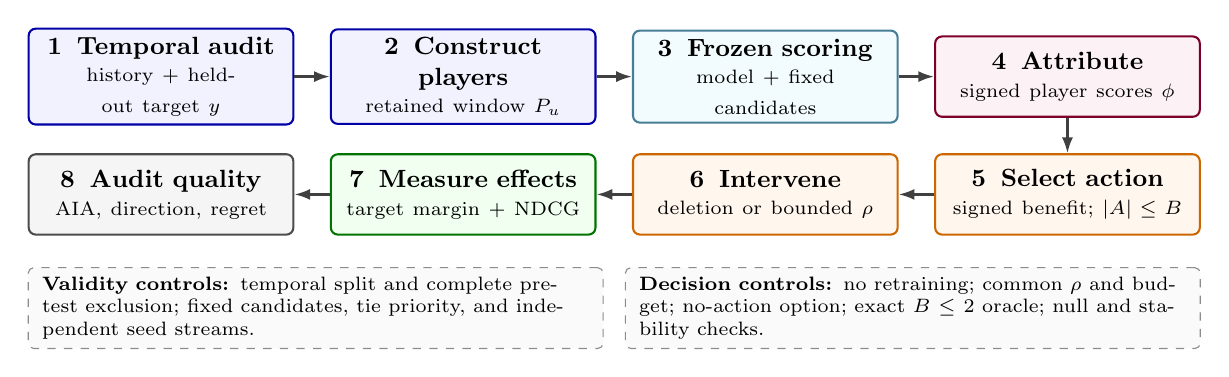
\begin{tikzpicture}[
  stage/.style={draw=black!70, fill=white, rounded corners=2.5pt,
    text width=3.15cm, minimum height=1.02cm, align=center,
    inner sep=3pt, font=\small, line width=.75pt},
  edge/.style={-{Latex[length=2mm,width=1.4mm]}, draw=black!75,
    line width=.85pt, rounded corners=2pt},
  control/.style={draw=black!45, dashed, fill=black!2, rounded corners=2pt,
    align=left, font=\scriptsize, inner xsep=5pt, inner ysep=3.5pt}
]
\node[stage, draw=blue!65!black, fill=blue!5] (a)
  {\textbf{1\enspace Temporal audit}\\[-1pt]\scriptsize history + held-out target $y$};
\node[stage, right=4.5mm of a, draw=blue!65!black, fill=blue!5] (b)
  {\textbf{2\enspace Construct players}\\[-1pt]\scriptsize retained window $P_u$};
\node[stage, right=4.5mm of b, draw=cyan!55!black, fill=cyan!5] (c)
  {\textbf{3\enspace Frozen scoring}\\[-1pt]\scriptsize model + fixed candidates};
\node[stage, right=4.5mm of c, draw=purple!65!black, fill=purple!5] (d)
  {\textbf{4\enspace Attribute}\\[-1pt]\scriptsize signed player scores $\phi$};

\node[stage, below=4.5mm of d, draw=orange!80!black, fill=orange!7] (e)
  {\textbf{5\enspace Select action}\\[-1pt]\scriptsize signed benefit; $|A|\le B$};
\node[stage, left=4.5mm of e, draw=orange!80!black, fill=orange!7] (f)
  {\textbf{6\enspace Intervene}\\[-1pt]\scriptsize deletion or bounded $\rho$};
\node[stage, left=4.5mm of f, draw=green!45!black, fill=green!6] (g)
  {\textbf{7\enspace Measure effects}\\[-1pt]\scriptsize target margin + NDCG};
\node[stage, left=4.5mm of g, draw=black!70, fill=black!4] (h)
  {\textbf{8\enspace Audit quality}\\[-1pt]\scriptsize AIA, direction, regret};

\draw[edge] (a.east)--(b.west);
\draw[edge] (b.east)--(c.west);
\draw[edge] (c.east)--(d.west);
\draw[edge] (d.south)--(e.north);
\draw[edge] (e.west)--(f.east);
\draw[edge] (f.west)--(g.east);
\draw[edge] (g.west)--(h.east);

\node[control, anchor=north west, text width=6.95cm]
  at ([yshift=-4mm]h.south west)
  {\textbf{Validity controls:} temporal split and complete pre-test exclusion; fixed candidates, tie priority, and independent seed streams.};
\node[control, anchor=north east, text width=6.95cm]
  at ([yshift=-4mm]e.south east)
  {\textbf{Decision controls:} no retraining; common $\rho$ and budget; no-action option; exact $B\le2$ oracle; null and stability checks.};
\end{tikzpicture}
\caption{ActionShap evaluation architecture for a retrospective, target-conditioned audit. The held-out temporal target $y$ defines the target-margin utility; the main path keeps player construction, frozen scoring, attribution, action selection, intervention, and outcome evaluation distinct. Control bands identify quantities fixed across explainers; stability diagnostics appear in the diagnostics tables in Supplementary Section~S8.}
\label{fig:architecture}
\end{figure}

\subsection{Attribution methods}
For a sampled base permutation $\pi_m$, let $S_{p,\pi_m}$ be the predecessor coalition of player $p$. We use $M_{\mathrm{pair}}$ base permutations and also evaluate each reverse order, giving $T=2M_{\mathrm{pair}}$ total prefix walks. The estimator is
\begin{equation}
\widehat\phi_{u,p}=\frac{1}{T}\sum_{t=1}^{T}\left[v_u^{\mathrm{attr}}(S_{p,\pi_t}\cup\{p\})-v_u^{\mathrm{attr}}(S_{p,\pi_t})\right].
\end{equation}
The exact value for reference is defined on the game $G_u=(P_u,v_u^{\mathrm{attr}})$ with $v_u^{\mathrm{attr}}(\varnothing)=0.5$, so efficiency sums to $v_u^{\mathrm{attr}}(P_u)-0.5$; it is
\begin{equation}
\phi^{\mathrm{exact}}_{u,p}=
\sum_{S\subseteq P_u\setminus\{p\}}
\frac{|S|!\,(n_u-|S|-1)!}{n_u!}
\left[v_u^{\mathrm{attr}}(S\cup\{p\})-v_u^{\mathrm{attr}}(S)\right].
\label{eq:exact-shapley}
\end{equation}
As a cooperative-game value, this exact expression satisfies efficiency, symmetry, dummy, and additivity; these classical properties are standard and are not re-derived. The reverse-paired estimator above is unbiased for this factorial-weighted value; it is used because $n_u$ can be too large for enumerating all $2^{n_u}$ coalitions. The reverse orders are reverse-paired samples used as a variance-reduction heuristic (reported as reverse pairing; a variance comparison against unpaired sampling is provided in the release), and the coalition-value cache is shared between a permutation and its reverse. In the executable configuration, \texttt{permutations} denotes $M_{\mathrm{pair}}=500$, hence $T=1000$ evaluated orders. The comparison includes locally weighted binary-mask LIME, LOO, greedy sequential deletion, and random attribution. No method observes measured intervention effects, oracle actions, or aggregate test outcomes.

For LIME, a binary mask $m_b\in\{0,1\}^{n_u}$ defines coalition $S_b=\{p:m_{b,p}=1\}$ and response $y_b=v_u^{\mathrm{attr}}(S_b)$. With normalized Hamming distance $d_b=n_u^{-1}\sum_p(1-m_{b,p})$, kernel width $\kappa=.25$, and ridge coefficient $\lambda_{\mathrm{LIME}}=1$, the fitted local surrogate is
\begin{equation}
(\hat\beta_0,\hat{\boldsymbol\beta})=\arg\min_{\beta_0,\boldsymbol\beta}
\sum_{b=1}^{512}\exp\left(-d_b^2/\kappa^2\right)\left(y_b-\beta_0-m_b^{\top}\boldsymbol\beta\right)^2
+\lambda_{\mathrm{LIME}}\lVert\boldsymbol\beta\rVert_2^2.
\label{eq:lime}
\end{equation}
The intercept is unpenalized and $\hat{\boldsymbol\beta}$ is the LIME attribution. The penalised least-squares problem is solved directly by closed-form ridge regression (deterministic; no iterative initialisation). The mask design contains the full, empty, and every leave-one-out mask; the remaining rows are independent Bernoulli$(0.5)$ masks (each history interaction retained with probability $1/2$), drawn from the attribution seed stream, which is independent of the model, candidate, tie, and user seeds. Masks are drawn with replacement: for short profiles the number of distinct coalitions is far below the design size ($2^5=32$ unique coalitions against $512$ rows at Amazon's median $n_u=5$), so repeated masks occur and the closed-form ridge fit implicitly weights each coalition by its multiplicity. We keep this identical seeded design at every history length for comparability and record it in the frozen configuration; enumeration-based and without-replacement mask designs are listed as a validation extension (Section~\ref{sec:limitations}).

For completeness, the greedy and random controls are defined operationally. Greedy sequential deletion starts at $S_0=P_u$. At step $t$ it evaluates $v_u^{\mathrm{attr}}(S_{t-1}\setminus\{p\})-v_u^{\mathrm{attr}}(S_{t-1})$ for every remaining player, selects the largest benefit, breaks ties by the lowest player index, records the signed value under the convention that $-\phi$ predicts downweight benefit, and recomputes the next step from the reduced coalition. It repeats until every player is ordered; it does not inspect bounded effects or the oracle, and the later signed action rule may abstain. Gradient-based attributions are available wherever the scoring path is differentiable with respect to the retained weights: finite-difference and integrated-gradient attributions along the weight path are evaluated in the replication subsection (Supplementary Section~S6) for both models, where they act as path-matched, intervention-aware baselines. Random attribution draws independent scores $r_{u,p}\sim\mathcal{N}(0,1)$ for every user and experiment seed using NumPy's seeded generator. The random vector is passed through the same signed action-selection rule as every explainer, including the same budget and abstention option. Its seed is independently offset from the model/attribution seed by $1{,}000{,}000+u$, so it is redrawn per user and seed.

\begin{algorithm}[t]
\caption{Greedy sequential-deletion baseline}
\label{alg:greedy-baseline}
\begin{algorithmic}[1]
\Require target-margin utility $v$, player set $P_u$
\Ensure signed ranking vector $\phi^{\mathrm{greedy}}_u$
\State $S\gets P_u$; recompute $v(S)$
\While{$S\ne\varnothing$}
  \State evaluate every $v(S\setminus\{p\})-v(S)$ for $p\in S$
  \State choose the maximum; break ties by lowest player index
  \State record its negative as $\phi^{\mathrm{greedy}}_{u,p}$; set $S\gets S\setminus\{p\}$
\EndWhile
\end{algorithmic}
\end{algorithm}

\begin{algorithm}[t]
\caption{Random attribution negative control}
\label{alg:random-baseline}
\begin{algorithmic}[1]
\Require user $u$, player count $n_u$, independent attribution seed $s$, budget $B$, strength $\rho$, common tie rule and abstention threshold
\Ensure random signed scores and optional action
\State draw $r_{u,p}\overset{\mathrm{iid}}{\sim}\mathcal{N}(0,1)$ for $p=1,\ldots,n_u$
\State apply the common signed downweight rule with budget $B$ and abstention
\State do not evaluate intervention effects before selecting the action
\end{algorithmic}
\end{algorithm}

\subsection{Metrics}
Let $\rho_S(\cdot,\cdot)$ denote Spearman rank correlation. Magnitude AIA is
\begin{equation}
\AIA_u^z(g)=\rho_S(|\phi^g_{u,p}|,|\Delta_{u,p}^{z,\mathrm{bnd}}|),\qquad z\in\{v_u^{\mathrm{attr}},q_u\}.
\label{eq:aia}
\end{equation}
Here and throughout, the superscript $g\in\{\mathrm{Shapley},\mathrm{LIME},\mathrm{LOO},\mathrm{Greedy},\mathrm{Random}\}$ indexes the attribution method. Deletion AIA substitutes $\Delta_{u,p}^{z,\mathrm{del}}$; bounded AIA uses $\Delta_{u,p}^{z,\mathrm{bnd}}$, and their difference is the bounded-minus-deletion magnitude-alignment difference (short: the gap). We use Spearman rank correlation rather than Pearson because the mapping from effects to utility is nonlinear (sigmoid margin, discrete NDCG) and heavy-tailed per-user effects would let a few extreme players dominate a linear correlation; Spearman also makes the metric invariant to monotone re-expressions of the utility. Kendall's $\tau$ is a rank-equivalent alternative and yields qualitatively identical orderings on these data; we retain Spearman for comparability with the deletion-evaluation literature. Signed alignment is $\rho_S(-\phi^g_{u,p},\Delta_{u,p}^z)$. For informative non-zero effects $I_u^z=\{p:\Delta_{u,p}^z\ne0\}$, direction accuracy is
\begin{equation}
\mathrm{DirAcc}_u^z(g)=|I_u^z|^{-1}\sum_{p\in I_u^z}\mathbf{1}\left[\operatorname{sign}(-\phi^g_{u,p})=\operatorname{sign}(\Delta_{u,p}^z)\right].
\end{equation}
We adopt $\operatorname{sign}(0)=0$; zero effects are excluded from $I_u^z$, so the value of $\operatorname{sign}(0)$ never contributes. When $I_u^z=\varnothing$, direction accuracy is missing. Let $k_u=\min(k,n_u)$ and let $T_{u,k_u}^g$ be the $k_u$ players with largest predicted benefit $-\phi^g$; top-$k$ intervention precision is reported for $k\in\{1,3,5\}$ in the release:
\begin{equation}
\mathrm{Prec}@k_u^z(g)=k_u^{-1}\sum_{p\in T_{u,k_u}^g}\mathbf{1}\left[\Delta_{u,p}^z>0\ \wedge\ \operatorname{sign}(-\phi^g_{u,p})=\operatorname{sign}(\Delta_{u,p}^z)\right].
\end{equation}
The indicator's sign condition is redundant given $\Delta>0$ and is kept for auditability; $\mathrm{Prec}@k$ is a fixed-$k$ diagnostic over the $k$ largest predicted benefits and is deliberately distinct from the abstention rule. If $n_u=0$ the quantity is missing. For a selected joint action $\widehat A_{u,g}$, success is $\mathbf{1}[\Delta_u^z(\widehat A_{u,g})>0]$; a negative realized effect identifies a harmful action, and abstention is $\mathbf{1}[\widehat A_{u,g}=\varnothing]$. Rank stability over $R_{\mathrm{seed}}$ seed runs is
\begin{equation}
\mathrm{Stab}_u(g)=\frac{1}{|V_u|}\sum_{(r,s)\in V_u}\rho_S(\boldsymbol\phi_{u}^{g,r},\boldsymbol\phi_{u}^{g,s}),\qquad V_u=\{(r,s):1\le r<s\le R_{\mathrm{seed}},\ \text{both vectors finite and nonconstant}\},
\end{equation}
computed only over finite nonconstant pairs; users with fewer than two such pairs are missing for this diagnostic.

For each user and seed, $R_{\mathrm{null}}=1{,}000$ within-seed permutations shuffle effect magnitudes across players. We first compute the observed AIA and its $R_{\mathrm{null}}$ null draws within each seed; then we average the observed value and each matched null draw across the five seeds within user. A user-level estimate requires at least three of five valid seed-level values; users with fewer are excluded and reported as missing. In the primary runs every retained user has all five seeds valid, and the seven Amazon users missing under every seed are excluded ($n=993$). Bootstrap and paired inference operate on these distinct-user summaries. The null test is a one-sided upper-tail test of alignment beyond chance, defined at the dataset level to match Table~5 exactly. For each valid user $u$, let $\bar A_u^{\mathrm{obs}}$ be the magnitude AIA averaged over the five seeds and $\bar A_u^{(r)}$ the matched seed-averaged null draw $r$ (effect magnitudes shuffled across players within each user and seed). With $U$ valid users,
\begin{equation}
p_{\mathrm{null}}=
\frac{1+\sum_{r=1}^{R_{\mathrm{null}}}\mathbf{1}\left[U^{-1}\textstyle\sum_u \bar A_u^{(r)}\ \ge\ U^{-1}\textstyle\sum_u \bar A_u^{\mathrm{obs}}\right]}{R_{\mathrm{null}}+1},
\label{eq:null-p}
\end{equation}
i.e.\ the dataset-level observed alignment is compared against the dataset-level null distribution of seed-averaged draws. The ten dataset--method null tests in Table~\ref{tab:aia-null} are unadjusted descriptive calibration controls (labelled ``Unadj.\ upper-tail null $p$''), not a confirmatory multiplicity family; confirmatory method comparisons use the Holm-adjusted paired tests of the statistical-validation tables in Supplementary Section~S8 and Supplementary Tables~S3--S5. We report null means, null 95th percentiles, plus-one permutation $p$-values, and valid-user counts. Constant vectors are missing, not imputed.

\FloatBarrier
\subsection{Decision quality and regret}
For a method action, define the additive predicted-benefit score
\begin{equation}
\widehat B_u^g(A)=-\sum_{p\in A}\widehat\phi_{u,p}^g.
\label{eq:predicted-benefit}
\end{equation}
This is an attribution-ranked additive decision heuristic, not a calibrated estimate of the realized joint effect. Realized pair effects may include interactions $I_{pq}=\Delta(\{p,q\})-\Delta(\{p\})-\Delta(\{q\})$ \cite{sundararajan2020shapleytaylor,janizek2021axiomatic}; Supplementary Section~S6 quantifies the resulting interaction error and evaluates an interaction-aware alternative that re-scores candidate pairs before selection, which changes the chosen action precisely when interactions are large (the SASRec runs). The additive rule is retained as the primary decision rule because it is the canonical budget-$B$ policy implied by any additive attribution and because it is the rule a practitioner would apply from an attribution vector alone; the eligibility threshold $\varepsilon=10^{-12}$ is a numerical zero tolerance that separates exactly-neutral candidates from sign-informative ones, and the results are insensitive to its value over $[10^{-15},10^{-6}]$ because signed effects are either identically zero or orders of magnitude larger. The method considers an action eligible when $\widehat B_u^g(A)>10^{-12}$; otherwise it abstains. Because this predicted benefit is additive, the implementation obtains the maximizer by sorting strictly positive individual benefits and taking at most $B$ of them; equal scores use the deterministic tie rule below. For utility $z$, the exact budget-two oracle is
\begin{equation}
A_u^{*,z}=\arg\max_{A\in\mathcal A_{u,2}}\Delta_u^z(A),
\end{equation}
and the method action is $\widehat A_{u,g}$. Because the no-action set belongs to $\mathcal A_{u,2}$, the oracle effect satisfies $\Delta_u^z(A_u^{*,z})\ge0$ by construction, so the normalized-regret denominator in Eq.~\eqref{eq:nregret} is only ever guarded against numerical zero, never negative. Regret is
\begin{equation}
\operatorname{Regret}_u^z(g)=\Delta_u^z(A_u^{*,z})-\Delta_u^z(\widehat A_{u,g}).
\end{equation}
For a general budget $B$, the utility-specific feasible oracle is
\begin{equation}
A_u^{*,z}(B)=\arg\max_{A\subseteq P_u,\,|A|\le B}\Delta_u^z(A).
\end{equation}
At $B=2$ the released primary results exhaustively enumerate no action, all singletons, and all pairs. The archived $B=3$ sensitivity was produced with the declared greedy lower-bound search rather than exhaustive triples; it is retained only for joint-effect, success, and abstention sensitivity. No normalized-regret claim is made for $B=3$. Exhaustive triples would require at most $1+20+\binom{20}{2}+\binom{20}{3}=1351$ actions per user and are recommended for a future regenerated $B=3$ release.

For utility $z$, normalized regret is
\begin{equation}
\operatorname{NRegret}_u^z(g)=
\frac{\Delta_u^z(A_u^{*,z})-\Delta_u^z(\widehat A_{u,g})}
{\Delta_u^z(A_u^{*,z})},
\qquad \Delta_u^z(A_u^{*,z})>\varepsilon,
\quad \varepsilon=10^{-12}.
\label{eq:nregret}
\end{equation}
It is averaged only over active-oracle users. Zero means an oracle-equivalent action; one means that the oracle improves the utility but the selected action achieves no improvement; values above one mean that the selected action is harmful. Values below zero are rejected by validation for the exact shared action space (up to floating-point tolerance); they would indicate an oracle or action-space inconsistency. The quantity is not clipped to one.

\begin{algorithm}[t]
\caption{Paired Monte Carlo attribution}
\label{alg:shapley}
\begin{algorithmic}[1]
\Require $u,P_u,v,M_{\mathrm{pair}}$, attribution seed
\Ensure $\widehat{\boldsymbol\phi}_u$
\State Initialise $\hat\phi_{u,p}\gets0$ for all $p\in P_u$
\For{$m=1$ to $M_{\mathrm{pair}}$}
\State Draw base order $\pi_m\sim\mathrm{Uniform}(\Pi(P_u))$; evaluate $\pi_m$ and its reverse as cached prefix walks
\For{each consecutive pair $(S,S\cup\{p\})$}
\State $\hat\phi_{u,p}\gets\hat\phi_{u,p}+v(S\cup\{p\})-v(S)$
\EndFor
\EndFor
\State Divide by $T=2M_{\mathrm{pair}}$ and record finite/constant-vector flags
\end{algorithmic}
\end{algorithm}

\begin{algorithm}[t]
\caption{Leakage-free signed action selection and exact budget-two oracle}
\label{alg:actions}
\begin{algorithmic}[1]
\Require attribution $\hat{\boldsymbol\phi}_u$, player set $P_u$, budget $B=2$, strength $\rho$, candidate set $E_u$, deterministic tie rule, utilities $z\in\{v_u^{\mathrm{attr}},q_u\}$; information set $\mathcal I_{\mathrm{select}}=\{\hat{\boldsymbol\phi}_u,P_u,\rho,B,\tau\}$ with $\Delta_u^z(A)\notin\mathcal I_{\mathrm{select}}$
\Ensure frozen method action, oracle actions, realized effects
\State \textbf{Stage 1 (selection, outcome-blind):} $\widehat B_u^g(A)\gets-\sum_{p\in A}\hat\phi_{u,p}$ for $A\in\mathcal A_{u,B}$
\State $\widehat A_{u,g}\gets$ argmax of eligible $\widehat B_u^g$ (deterministic tie rule); $\widehat A_{u,g}\gets\varnothing$ if best score $\le10^{-12}$
\Statex\hspace{1em}\textit{(additive unit-cost scoring makes sorting positive individual benefits equivalent to enumerating $\mathcal A_{u,B}$; the additive score is a decision heuristic, not a consequence of Shapley theory)}
\State \textbf{FREEZE} $\widehat A_{u,g}$
\State \textbf{Stage 2 (outcome evaluation, after freezing):} for $A\in\{\varnothing\}\cup$ singletons $\cup$ unordered pairs: construct $w^{A,\rho}$ and compute $\Delta_u^z(A)$ for every $z$
\State $A_u^{*,z}\gets\arg\max_A\Delta_u^z(A)$ with cardinality-then-lexicographic tie rule
\State \Return $\widehat A_{u,g}$, $\{A_u^{*,z}\}_z$, $\{\Delta_u^z(A)\}_{A,z}$
\end{algorithmic}
\end{algorithm}

Equal action scores use a deterministic common rule: maximize predicted benefit first; among ties choose the smaller action cardinality; among equal-cardinality ties choose the lexicographically lower sorted player-index tuple. An abstention action wins when the best predicted benefit is at most $10^{-12}$. The exact oracle uses the same cardinality and lexicographic rule after maximizing realized utility.

\begin{algorithm}[t]
\caption{Distinct-user inference and AIA null}
\label{alg:inference}
\begin{algorithmic}[1]
\Require Five seed records per user and $R_{\mathrm{null}}=1000$ null draws per seed
\Ensure User-level estimates and corrected comparisons
\For{each distinct user $u$ and seed $s$}
\State Compute seed-level AIA only for finite, nonconstant vectors
\For{$r=1$ to $R_{\mathrm{null}}$}
\State Shuffle effect magnitudes within $(u,s)$; recompute the null AIA
\EndFor
\EndFor
\For{each distinct user $u$}
\State Require at least three of five valid seed-level values, else mark missing
\State Average the observed AIA and each matched null draw across valid seeds
\EndFor
\State Bootstrap distinct users ($R_{\mathrm{boot}}=10{,}000$); for each declared paired comparison run $R_{\mathrm{perm}}=10{,}000$ sign permutations, plus-one two-sided $p$, Holm correction within the explicitly named dataset--model--condition--metric family
\end{algorithmic}
\end{algorithm}

\begin{algorithm}[t]
\caption{Independent convergence selection}
\label{alg:convergence}
\begin{algorithmic}[1]
\Require $M_{\mathrm{pair}}\in\{25,50,100,250,500,1000\}$ and an independent $M_{\mathrm{pair}}=1000$ reference
\Ensure Selected $M_{\mathrm{pair}}$ or explicit unconverged status
\For{each candidate $M_{\mathrm{pair}}$}
\State For each candidate $M_{\mathrm{pair}}$, evaluate $T=2M_{\mathrm{pair}}$ forward/reverse orders and compare attribution ranks and signed-$B=2$ action Jaccard with the independent reference
\State Record rank-valid fraction and threshold coverage
\EndFor
\State Select smallest $M_{\mathrm{pair}}$ whose population means satisfy rank $\ge.95$, Jaccard $\ge.80$, rank validity $\ge.95$ (a population-average diagnostic; per-user coverage is reported separately, so conditions are labelled mean-converged rather than user-universally converged)
\If{no candidate qualifies}\State Retain $M_{\mathrm{pair}}=1000$ as an unconverged stress test\EndIf
\end{algorithmic}
\end{algorithm}

\section{Experimental Protocol}
\subsection{Datasets and temporal split}
The selected evaluation cohort comprises $1{,}000$ users per dataset drawn with user seed $2718$ from the eligibility pool of test users with at least four training interactions: $6{,}028$ eligible users on MovieLens-1M and $7{,}621$ on Amazon Digital Music, so the cohort is a seeded subsample of a fully enumerated pool rather than an identifier-ordered prefix, and every sampled user satisfies the four-interaction floor (the four-interaction floor counts training, validation, and test events, so the minimum possible player count after reserving validation and test is two; the observed minimum is three). Retained history lengths differ sharply between domains (MovieLens median/IQR $20/20$ events at the $n_{\max}$ cap, Amazon $5$/$3$--$8$, reflecting its sparsity); per-step filtering counts are recorded in the release dataset audit.
\safeinput{tables/profile_window_audit.tex}
The audit table makes the cohort asymmetry explicit: most MovieLens users sit at the $20$-player boundary, whereas the median Amazon user has five players and only $5.9\%$ reach the cap. Cross-dataset contrasts are therefore interpreted descriptively, and Section~\ref{sec:robustness} reports a history-stratified analysis rather than attributing the larger Amazon difference to dataset identity alone.
We use MovieLens-1M \citep{harper2016} and Amazon Digital Music reconstructed from the Amazon Reviews 2018 release \citep{ni2019}. Positive feedback is rating $\ge4$; Amazon duplicate user--item records retain the latest deterministic event and iterative 5-core filtering is reapplied after thresholding. MovieLens retains 6,035 users, 3,533 items, and 575,276 positive interactions. Amazon retains 10,623 users, 8,582 items, and 104,431 interactions. Source and processed hashes are recorded in the final manifest.

\subsection{Models, candidates, and gates}
The matrix includes ItemKNN and profile aggregation, five seeds, primary 1,000-user sampled ranking, 250-user full-catalogue subsets, and declared history, candidate, intervention-strength, budget, and utility sensitivities. ItemKNN uses cosine item--item similarities from binary training histories, removes self-similarity, retains the 200 largest non-zero neighbours per item, and applies no shrinkage or minimum-support threshold beyond the observed co-occurrence counts; all retained similarities are non-negative. The profile robustness model uses 64-dimensional item embeddings, ten leave-one-out BPR-style epochs, one sampled positive per user per epoch, uniform negatives outside the complete training history, learning rate $0.03$, and $L_2$ coefficient $10^{-4}$. Both models recompute the profile from the retained player window at inference time and are not retrained under an intervention.

The primary candidate set contains the target and 199 uniformly sampled unseen negatives. Candidate seed $1729$, user seed $2718$, tie seed $31415$, and model/attribution seeds $42$--$46$ are independent. The masking gate is defined as follows: for 200 gate users (seeded subsample) on a fixed 200-item sampled candidate set, exactly one uniformly chosen player is deleted per user; the gate passes for a model seed if (i) the top-10 order changes for at least $50\%$ of gate users, (ii) the mean absolute NDCG@10 change is at least $10^{-3}$, and (iii) a frozen-score static control is exactly invariant to the mask argument (verifying that only the retained-history path carries information). ItemKNN passes all blocking masking gates on every seed. The profile model fails the NDCG masking threshold for one MovieLens seed (mean absolute change $0.000682$ versus $0.001$) and is retained as a nonblocking robustness boundary.

LIME uses 512 binary masks including the full, empty, and all leave-one-out masks, a normalized Hamming-distance kernel with width $0.25$, and ridge coefficient $1.0$. The target-margin competitor count is $L=10$ and the sigmoid temperature is one. The primary intervention is $\rho=0.5$; $\rho=0.25$ is sensitivity-only. The exact budget-two action space includes no action, all singletons, and all pairs.

\subsection{Statistical analysis}
For each seed we compute user-level quantities first; repeated seed values are then averaged within distinct user before bootstrap resampling. A user summary requires at least three of five valid seed-level values; users with fewer valid seeds are excluded and counted as missing (in the primary runs all retained users have five valid seeds, and seven Amazon users are missing under every seed). User bootstrap intervals are two-sided percentile intervals from 10,000 user resamples. For a paired metric, $d_u=x_u-y_u$ and $T_{\mathrm{obs}}=n^{-1}\sum_{u=1}^{n}d_u$. Paired plus-one sign permutations use 10,000 two-sided sign flips $T_r^*=n^{-1}\sum_u\epsilon_{u,r}d_u$, with $\epsilon_{u,r}\in\{-1,+1\}$ and $p=(1+\#\{|T_r^*|\ge|T_{\mathrm{obs}}|\})/(R+1)$. Holm correction is applied separately within each dataset--model--condition--metric family across the declared method-pair comparisons. Paired Cohen's $d_z$ is $\bar d/s_d$, where $d_u$ is the user-level paired difference and $s_d$ its sample standard deviation. The paired comparison uses the intersection of users with finite values for both methods; missing correlations are retained as missing. Active-oracle counts define the denominator for normalized regret. No coalition evaluation is an independent statistical observation.
Three further checks frame the confirmatory family. First, a Friedman omnibus test over the five methods' user-level bounded AIA rejects equal distributions on both datasets ($\chi^2=3767.2$ on MovieLens, $2482.0$ on Amazon; both $p<10^{-300}$ at $n\ge993$), justifying the subsequent pairwise comparisons. Second, paired Cohen's $d_z$ is reported with every Holm-adjusted comparison in the release; for the headline alignment contrasts it is large ($d_z=-1.010$ Shapley--LIME and $-1.254$ Shapley--LOO on MovieLens; $-0.726$ and $-0.771$ on Amazon), while for realized-NDCG contrasts it is small ($|d_z|\le0.085$). Third, a post-hoc minimum-detectable-effect analysis at 80\% power shows the 1,000-user cohort resolves bounded-AIA differences of $\pm0.014$ (MovieLens) and $\pm0.051$ (Amazon), but resolves NDCG-effect differences only to $\pm0.002$--$0.004$; the observed decision-quality differences ($\le0.003$) therefore fall at or below the detectable threshold, so non-detection of decision-quality differences is a power statement, not an equivalence claim (the TOST equivalence result for Amazon Shapley--LIME uses an independently declared margin).

\subsection{Reproducibility}
The real result archive contains 80 recommendation runs plus five convergence studies. All assets in this manuscript are generated from schema-v2 raw results with repository-relative paths and content hashes. The primary ItemKNN target-margin analysis uses $M_{\mathrm{pair}}=500$ base permutations and $T=1000$ evaluated orders; the independent convergence study selects lower diagnostic values for some conditions, while the conservative final floor is retained. The archived runs record macOS-26.5.1-arm64, Python 3.12.13, NumPy 2.4.6, SciPy 1.17.1, pandas 2.3.3, scikit-learn 1.9.0, matplotlib 3.11.1, and PyYAML 6.0.3. Historical processor model, RAM, and peak RSS were not serialized.

\section{Results}\label{sec:results}
All numerical claims below are generated only when \texttt{validation\_report.json} reports PASS. The legacy pilot is excluded from the canonical package.

\subsection{Recommendation quality and protocol audit}
Table~\ref{tab:recommendation-quality} shows that primary ItemKNN exceeds the popularity reference on both datasets. MovieLens ItemKNN reaches NDCG@10 $=0.284$ and HitRate@10 $=0.504$, compared with $0.158$ and $0.320$ for popularity. Amazon ItemKNN reaches $0.181$ and $0.285$, compared with $0.090$ and $0.155$. The profile model is weaker on both datasets and is therefore interpreted only as architectural robustness evidence.

Because each user has one held-out target, sampled-set HitRate@10 is numerically the same indicator as a one-target recall measure; HitRate is used here to avoid any implication of catalogue-level retrieval recall.

\safeinput{tables/recommendation_quality.tex}
\FloatBarrier

\subsection{Faithfulness versus bounded alignment}
Table~\ref{tab:aia-components} separates deletion AIA, bounded AIA, and their difference. On MovieLens ItemKNN, Shapley has bounded AIA $0.779$ versus $0.933$ for LIME and $0.978$ for LOO. On Amazon, Shapley has bounded AIA $0.414$ versus $0.827$ and $0.851$. Thus Shapley does not win absolute alignment. This conclusion is estimator-robust: replacing the reverse-paired Monte Carlo estimator with KernelSHAP at LIME's mask budget (256/512 masks) leaves bounded alignment at $0.65$--$0.66$ on MovieLens and $0.63$ on Amazon, far below LIME and LOO in either case, and the two Shapley estimators agree strongly (Pearson $0.78$--$0.98$; Supplementary Table S15).

The contrast is in the change between perturbations. Shapley’s primary gap is $+0.0169$ on MovieLens and $+0.1285$ on Amazon. LIME and LOO are negative. The random control is close to zero and its confidence intervals include zero in the primary conditions. Greedy is negative on the primary conditions. The gap therefore measures a change of evaluation target; it is not an explanation-validity score.

\begin{figure}[pos=t]
\centering
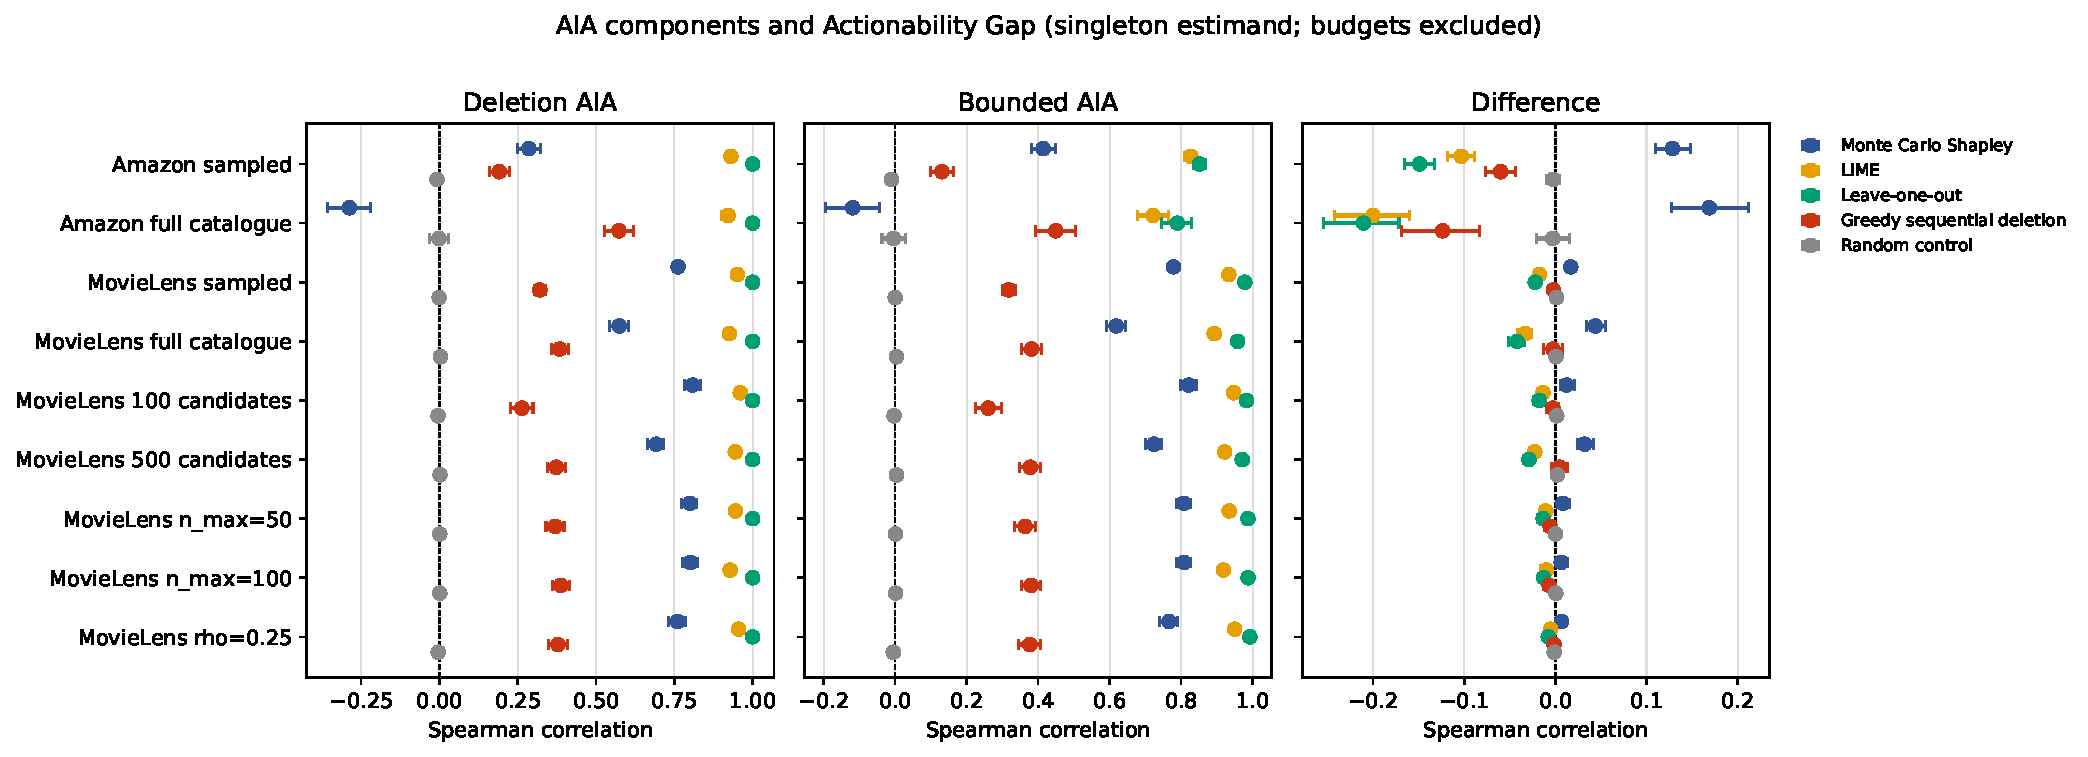
\includegraphics[width=\linewidth]{aia_components_robustness.pdf}
\caption{Deletion AIA, bounded-intervention AIA, and their difference for the five methods. Points are distinct-user means and intervals are user-bootstrap 95\% confidence intervals. Budget rows are excluded because budgets do not define singleton gap estimands. The underlying values are also supplied in editable Table~\ref{tab:aia-components} and the alignment table in Supplementary Section~S7, so interpretation does not depend on color alone.}
\label{fig:aia-components}
\end{figure}

\safeinput{tables/aia_components.tex}
\FloatBarrier

\subsection{Joint intervention decisions}
The operational outcome is NDCG@10 under the exact $B=2$ action space. On MovieLens ItemKNN, LOO yields mean NDCG effect $0.0431$, LIME $0.0425$, and Shapley $0.0403$. Success is $28.9\%$, $28.8\%$, and $27.4\%$, respectively. Conditional normalized regret among 339 active-oracle users is $0.217$, $0.225$, and $0.268$. Local methods therefore retain a modest decision advantage on MovieLens.

On Amazon ItemKNN, NDCG effects are $0.0333$ for Shapley, $0.0331$ for LIME, and $0.0313$ for LOO. Conditional normalized regret among 196 active-oracle users is $0.206$, $0.197$, and $0.232$. The differences are small and do not support a universal winner. Random actions have negative mean NDCG effects on both datasets. Signed alignment---the Spearman correlation between predicted benefits $-\phi^g_{u,p}$ and bounded effects $\Delta^{z,\mathrm{bnd}}_{u,p}$, distinct from direction accuracy (Eq.~17)---is high for the gradient-consistent methods and collapses for the controls (Table~\ref{tab:app-diagnostics}: Amazon $0.855$ Shapley, $0.949$ LIME, $0.966$ LOO, $0.109$ Greedy, $0.009$ Random; MovieLens $0.929$, $0.974$, $0.994$, $0.342$, $0.004$), so the magnitude-alignment ordering transfers to sign validity.

For the Amazon Shapley-versus-LIME realized-NDCG comparison we declare a practical equivalence margin of $\pm0.005$ $\Delta$NDCG as the smallest decision-relevant effect size (approximately one eighth of the typical realized effect magnitude $0.04$) and apply TOST on the seed-averaged paired user differences ($n=993$ on Amazon after constant-vector exclusion): the mean difference is $+0.00013$ with 90\% CI $[-0.00162,+0.00188]$ entirely inside $\pm0.005$ (both one-sided $p<10^{-4}$), so the two methods are practically equivalent on Amazon realized NDCG under this margin; we therefore report equivalence within a declared margin rather than interpreting a nonsignificant test as indistinguishability. On MovieLens the same test also falls inside $\pm0.005$ (mean $-0.00227$, 90\% CI $[-0.00365,-0.00088]$) while excluding zero, i.e.\ LIME is detectably but practically slightly better. Normalized regret is right-skewed: medians are $0$ for Shapley/LIME/LOO (fraction above one $\le0.3\%$), whereas Greedy reaches the $95$th percentile $2.81$ on MovieLens ($15.9\%$ of users above one) and Random $3.39$ ($33.0\%$), so mean regret differences are driven by a harmful-action tail that the signed, abstention-aware rule avoids.

\safeinput{tables/intervention_outcomes.tex}

\begin{figure}[pos=t]
\centering
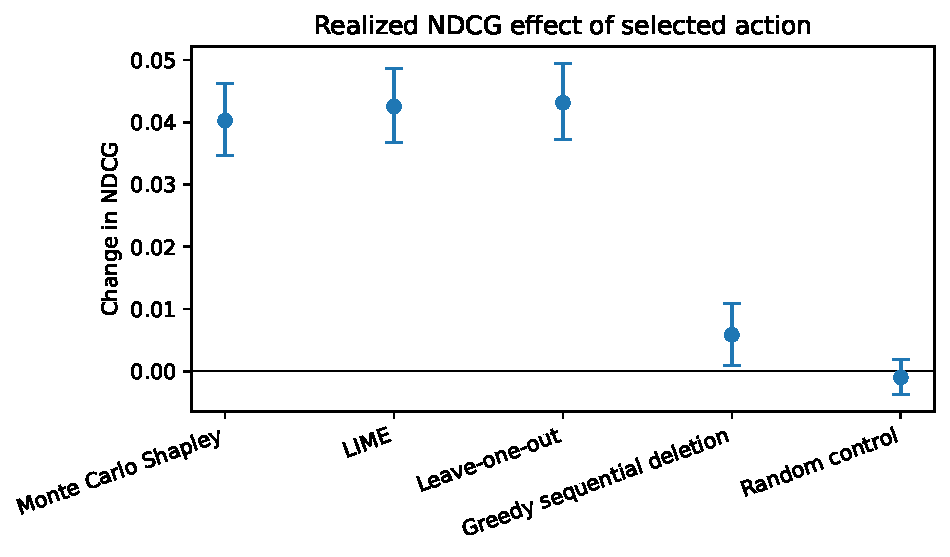
\includegraphics[width=\linewidth]{joint_ndcg_MovieLens-1M_itemknn_sampled_unseen_negatives_with_target_target_margin_primary_primary.pdf}
\caption{Primary MovieLens ItemKNN NDCG effect for actions selected at budget two. We show MovieLens for visual legibility; the analogous Amazon effects are reported in Table~\ref{tab:intervention-outcomes}. The comparison is retrospective and target-conditioned; intervals are distinct-user bootstrap intervals.}
\label{fig:joint-ndcg}
\end{figure}
\FloatBarrier

\subsection{Hypothesis adjudication}
The two predeclared hypotheses are adjudicated here against the primary results. \textbf{H1} (deletion and bounded interventions probe distinct, method-specific response surfaces) is supported: the bounded-minus-deletion gaps in Table~\ref{tab:aia-components} are non-zero and method-specific---positive for Shapley ($+0.017$ MovieLens, $+0.129$ Amazon, bootstrap CIs excluding zero), negative for LIME ($-0.018$, $-0.103$) and LOO ($-0.022$, $-0.149$)---so the ordering of methods changes with the perturbation semantics. \textbf{H2} (pointwise alignment does not determine decision quality) is also supported: LIME and LOO dominate Shapley on absolute bounded alignment yet the realized-NDCG differences among the three methods are small, dataset-inconsistent, and---on Amazon---within the declared equivalence margin (Section~\ref{sec:results}). The predeclared falsification check asks whether the gap predicts decision quality: it does not. Across users, the Spearman correlation between the bounded-minus-deletion gap and normalized regret is $+0.035$ ($p=0.27$, $n=1000$) on MovieLens and $+0.042$ ($p=0.19$, $n=987$) on Amazon for Shapley, and the correlation with realized NDCG effect is $-0.054$ ($p=0.085$) and $-0.097$ ($p=0.002$) respectively; nothing here supports reading a positive gap as decision-relevant, which is why the gap is reported only as a perturbation-sensitivity diagnostic.

\subsection{Null calibration and convergence}
Table~\ref{tab:aia-null} reports the complete within-user null calibration alongside the component table. The within-user AIA null is centred near zero for all primary ItemKNN conditions, and Shapley, LIME, LOO, and greedy sequential deletion exceed the null for bounded magnitude AIA, while random attribution does not. This establishes that bounded alignment is not merely a consequence of the correlation statistic returning positive values.
\FloatBarrier
\safeinput{tables/aia_permutation_null.tex}

Exact enumeration is feasible only for short profiles: the 250-user replication runs enumerate $89$/$87$ users with $n_u\le12$ on Amazon (ItemKNN/SASRec) and $6$/$8$ on MovieLens, whose histories are longer, while a dedicated validation on the 1,000-user primary cohort enumerates $300$ Amazon and $73$ MovieLens users (Supplementary Section~S9); the two counts refer to these different cohorts. Both show model- and dataset-dependent agreement of the reverse-paired estimator: MovieLens ItemKNN reaches a mean per-user maximum absolute error of $2.1\times10^{-3}$ with mean rank agreement $\rho=0.982$, whereas Amazon ItemKNN reaches $1.1\times10^{-4}$ but only $\rho=0.783$; under SASRec the corresponding mean agreements are $\rho=0.688$ (MovieLens) and $\rho=0.395$ (Amazon). A small absolute error therefore does not imply high rank agreement when the exact attribution spectrum is compressed or nearly tied, and Monte Carlo accuracy is validated separately per dataset and architecture.

Under the population-average diagnostic criteria, target-margin convergence selects $M_{\mathrm{pair}}=50$ for Amazon ItemKNN, $M_{\mathrm{pair}}=100$ for Amazon profile, $M_{\mathrm{pair}}=250$ for MovieLens ItemKNN, and $M_{\mathrm{pair}}=50$ for MovieLens profile, with per-user joint-threshold coverage at the selected budgets of $0.56$--$0.69$ (rising to at most $0.89$ at $M_{\mathrm{pair}}=1000$, and $0.74$--$0.85$ at the $500$--$1000$ floor in the quantile table of Supplementary Section~S8); these settings are therefore mean-converged and are conservatively overridden by the final floor $M_{\mathrm{pair}}=500$ ($T=1000$ evaluated orders). Rank-valid fraction is the fraction of users with finite rank comparisons, whereas threshold coverage is the fraction of rank-valid users satisfying both the rank and action-overlap thresholds; coverage is diagnostic and is not a replacement for the rank-validity criterion. The NDCG attribution sensitivity remains unconverged at $M_{\mathrm{pair}}=1000$ and is reported only as a stress test.

\safeinput{tables/convergence.tex}

\begin{figure}[pos=t]
\centering
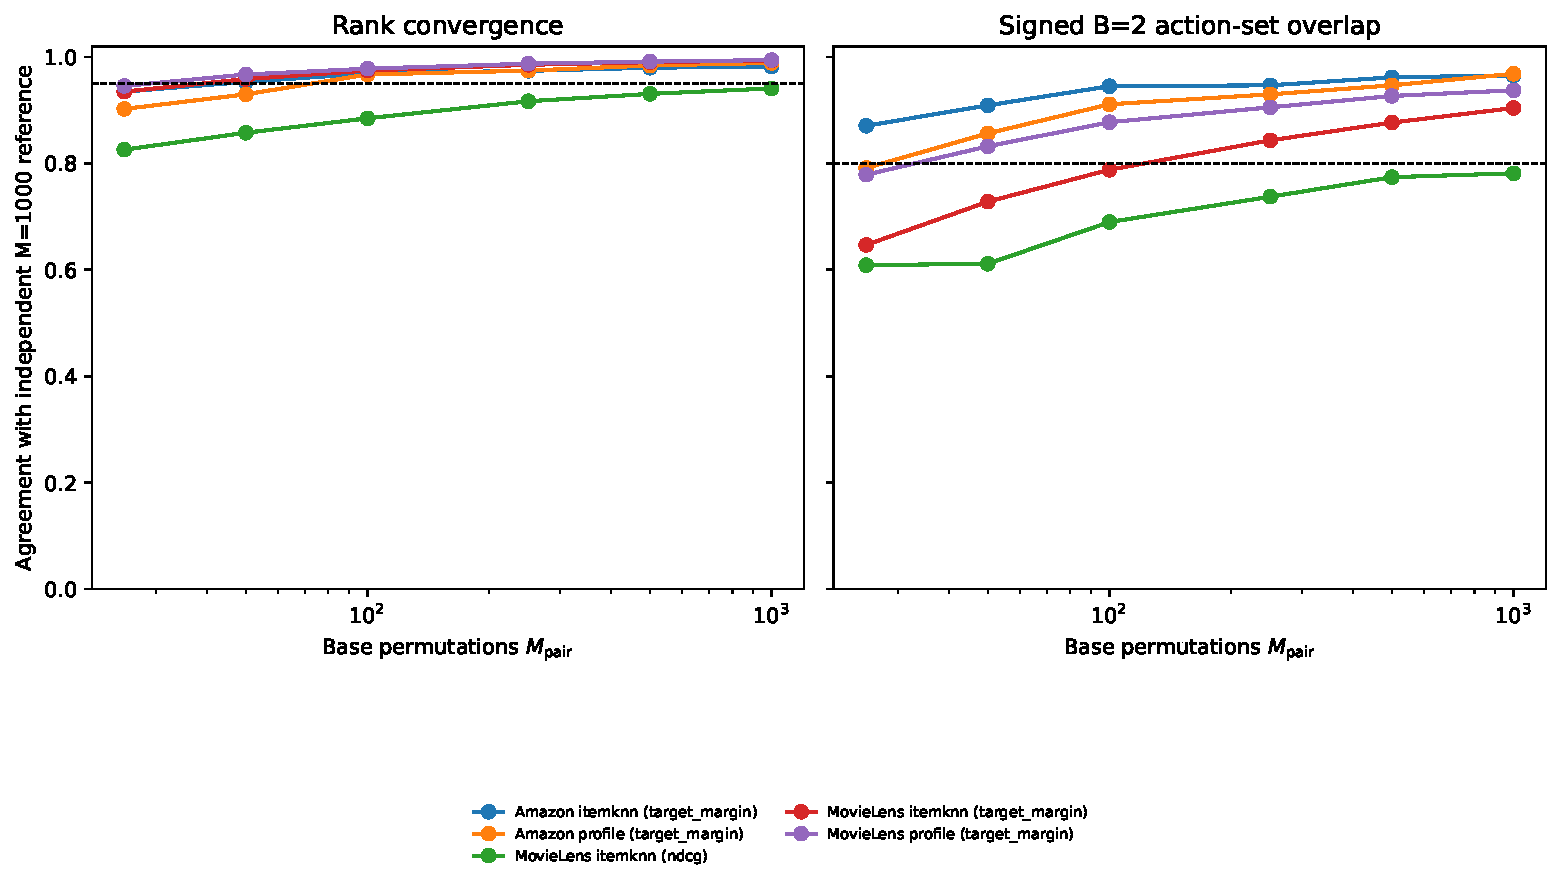
\includegraphics[width=\linewidth]{convergence.pdf}
\caption{Independent Monte Carlo convergence against an independent $M_{\mathrm{pair}}=1000$ \emph{MC reference} (not ground truth; an exact-reference subset is specified in the replication guide). Left: rank agreement with the reference; right: signed $B=2$ action-set Jaccard overlap, the second selection criterion; dashed lines mark the $0.95$ and $0.80$ thresholds. The legend maps every curve to its dataset--model--utility condition. The numerical values are provided in Supplementary Table~S6, so interpretation does not rely on colour alone. Efficiency is not used as a convergence criterion because the prefix walk telescopes.}
\label{fig:convergence}
\end{figure}
\FloatBarrier

\subsection{Robustness and boundaries}\label{sec:robustness}
Before reporting the sensitivities we state their interpretive ceiling. Scaling the Amazon full-unseen-catalogue audit from 250 to the full 1,000-user cohort (median catalogue $8{,}572$ unseen items; Table~\ref{tab:review5-fullcat}) raises the number of active target-margin oracles to $883$. At catalogue scale, LIME and leave-one-out retain positive bounded alignment ($0.71$ and $0.78$) while Monte Carlo Shapley is mildly anti-aligned ($-0.050$) despite a positive bounded-minus-deletion difference ($+0.16$); the difference therefore again reflects reduced anti-alignment rather than successful bounded-intervention prediction. Full-catalogue decision effects are near zero for every method, so catalogue-scale decision conclusions remain descriptive. With that caveat, the bounded-minus-deletion difference for Shapley stays positive across the primary ItemKNN candidate, history, and intervention-strength conditions, while absolute values vary. Full-catalogue NDCG alignment is sparse ($54$ active NDCG oracles) and is treated descriptively. The longer-history conditions also show reduced masking sensitivity, supporting the use of $n_{\max}=20$ as a declared operating boundary rather than an arbitrary computational cap.

\safeinput{tables/review5_full_catalogue.tex}

The profile model supplies a useful negative boundary: it can change rankings while underperforming popularity, and one MovieLens seed fails the NDCG masking threshold. This demonstrates why a non-degenerate masking gate and recommendation-quality audit are necessary before interpreting attribution results.

\safeinput{tables/history_stratified_gap.tex}

History length explains part, but not all, of the cross-dataset contrast (Table~\ref{tab:history-stratified-gap}). The Amazon Shapley difference remains positive in every history stratum, including $n_u=20$; MovieLens is also positive, although its dominant $n_u=20$ stratum has a smaller mean difference. The nine-user MovieLens $3$--$5$ stratum is too small for a stable cross-dataset comparison and is flagged in the table caption. Accordingly, ``especially on Amazon'' is reported as a descriptive empirical pattern rather than a dataset-causal conclusion.


A replication of selected audit components under a nonlinear sequential scorer (a SASRec-style transformer) is reported in Supplementary Section~S6, together with the intervention-aware (path-matched) baselines and the prospective, non-target-conditioned audits. Its headline findings are that path-matched baselines match or exceed Monte Carlo Shapley when pair interactions are strong, that prospective audits leave the alignment conclusions intact, and that the signed, abstention-aware selection rule is supported by the component ablation. Beyond this, the central alignment finding generalizes: path-matched baselines (finite differences, integrated gradients, bounded LIME) exceed Monte Carlo Shapley on bounded-intervention alignment under a graph architecture (LightGCN) and on a third dataset from a different domain (Gowalla location check-ins), as detailed in Supplementary Section~S10.

\section{Discussion and Broader Implications}
The results support a three-axis interpretation. LIME and LOO are strongest on absolute pointwise alignment because their constructions are local to deletion or the full profile. Shapley has lower absolute alignment but a larger positive change when the evaluation moves from deletion to bounded downweighting. This is consistent with coalition-context averaging, but the experiment does not establish a causal mechanism and the random control prevents interpreting the gap as standalone validity.

Table~\ref{tab:related-work-comparison} compares the protocol dimensions most relevant to the closest counterfactual and explanation-evaluation studies. The five criteria (player type, intervention policy, outcome, joint oracle, inference) were chosen because they are exactly the dimensions that determine whether an explanation-evaluation protocol can audit attributions against feasible, budgeted, joint decisions with statistically valid user-level evidence.

ActionShap is an evaluation protocol, not a counterfactual generator or attribution algorithm: every explainer is audited against the same declared bounded intervention policy and exact action space, after which singleton alignment and joint decision regret are measured with abstention permitted and inference performed over distinct users with an explicit chance control. Relative to the closest work (Table~\ref{tab:related-work-comparison}), including recent counterfactual-explanation benchmarks and studies showing that recommender performance itself alters explainer evaluation \cite{mohammadi2024recsys,nguyen2026}, the non-overlap is the combination of bounded intervention semantics, null-calibrated attribution alignment, and exact joint-action regret under a common feasible space.

\begin{table}[t]
\centering\scriptsize
\caption{Component-level positioning against the closest related evaluation and counterfactual recommendation work.}
\label{tab:related-work-comparison}
\setlength{\tabcolsep}{2pt}
\begin{tabularx}{\linewidth}{@{}>{\raggedright\arraybackslash}p{.14\linewidth}*{7}{>{\raggedright\arraybackslash}X}@{}}
\toprule
Work & Players & Policy & Outcome & Oracle & Inference & Bounded/cont. & Null ctrl. \\
\midrule
PRINCE \cite{ghazimatin2020} & Provider, profile & Counterfactual gen. & Rec.\ change & Method-spec. & Method-spec. & No & No \\
ACCENT \cite{tran2021} & User factors & Counterfactual masking & Top-$K$ expl. & None & Method-spec. & No & No \\
Tan et al. \cite{tan2021} & Rec.\ factors & Counterfactual expl. & Rank change & Method-spec. & User/item & No & No \\
CEERS \cite{baklanov2024} & Expl.\ factors & Counterfactual eval. & Expl.\ quality & Benchmark & Repro. & No & No \\
Barkan \cite{barkan2024} & Learned masks & Model-spec.\ cf. & Expl.\ quality & Learned & Method-spec. & Learned & No \\
LXR \cite{gurevitch2025} & Learned masks & Model-spec.\ cf. & Expl.\ quality & Learned & Method-spec. & Learned & No \\
Mohammadi \cite{mohammadi2025} & Expl.\ factors & Top-$K$ cf.\ eval. & Consistency & None & Benchmark & No & No \\
Nguyen \cite{nguyen2026} & User/profile & Top-$K$ cf.\ eval. & Effect., sparsity & Benchmark & Cross-paper & No & No \\
RankSHAP \cite{chowdhury2024rankshap} & Rank features & Attribution & Rank fidelity & None & Feature-level & No & No \\
ShaRP \cite{pliatsika2025sharpl} & Rank elements & Attribution & Rank preference & None & Feature-level & No & No \\
TimeSHAP \cite{bento2021timeshap} & Sequence events & Event deletion & Sequence output & None & Feature-level & No & No \\
Ref.\ fidelity \cite{baklanov2025fidelity} & Expl.\ factors & Cf./deletion & Fidelity & Benchmark & Benchmark & No & No \\
CLIME \cite{mousavi2023clime} & Features & Deletion & Local fidelity & None & Feature-level & No & No \\
Session attr.\ \cite{bruun2025session} & Session events & Deletion & Session ranking & None & Feature-level & No & No \\
ActionShap & History interactions & Bounded downweight & AIA, NDCG, regret & Exact $B=2$; abstain & Distinct-user & Binary+cont. & Within-user \\
\bottomrule
\end{tabularx}
\end{table}

The decision results reinforce this distinction. On MovieLens, local methods select slightly better NDCG actions. On Amazon, Shapley and LIME are close, with modest differences in conditional regret. A method can therefore show a positive change between deletion and bounded-intervention alignment without selecting the best action for every operational utility. This is precisely why ActionShap reports pointwise alignment, signed direction, success, abstention, and regret together.

When should a practitioner use this protocol instead of a deletion audit? Consider a platform that can discount suspect historical interactions---suspected bot clicks, stale preferences, or disputed ratings---but cannot delete them, so the executable policy is a bounded downweighting at some operating strength. A deletion audit ranks interactions by their removal effect; if the operational policy is bounded, that ranking can misestimate which interactions actually move the recommendation, because deletion and bounded downweighting probe different response surfaces (Section~\ref{sec:robustness} shows methods re-ranking between the two semantics). ActionShap answers three concrete questions a deletion audit cannot: (i) does this attribution predict bounded intervention effects at the operating strength (bounded AIA and signed directional accuracy); (ii) would acting on it select a near-oracle joint action under the declared budget (regret against the exact oracle); and (iii) are these conclusions distinguishable from chance for this user population (within-user null calibration)? A positive bounded-minus-deletion gap is not itself a decision criterion---the results show it does not select better actions---but it flags exactly the settings in which deletion-based conclusions are fragile, which is when a bounded audit is worth running.
The protocol also clarifies what offline actionability means. The intervention is system-executable inside the frozen simulator: it changes an inference-time interaction weight without retraining. It is not automatically a user action, causal intervention, or prospective policy. A production deployment would need authority, cost, user-consent, and feedback-loop specifications that are outside this benchmark.

From a responsible-AI standpoint, ActionShap is an oversight instrument rather than a deployment policy: it makes explicit which attributions correspond to feasible, predictable changes under a declared policy, and it treats a positive bounded-minus-deletion difference as descriptive rather than as evidence of user-facing actionability, preventing the failure mode in which faithful-but-unactionable explanations are consumed as operational advice. This supports transparency and human-oversight objectives of trustworthy-AI frameworks without claiming perceived usefulness, which remains outside the benchmark's scope.

\subsection{Limitations and Threats to Validity}\label{sec:limitations}
\subsubsection{Construct validity}
Actionability is defined as predictive validity under one bounded downweighting policy. It is not perceived usefulness, legal recourse, user agency, or a causal effect in the world. All primary players are technically mutable, so feasibility does not differentiate factors; future work should study heterogeneous costs and user-side constraints.

\subsubsection{Metric validity}
NDCG is discrete and produces constant effect vectors for some users. We report missing correlations rather than imputing zero. Target margin is the converged attribution utility but has less direct operational meaning; NDCG is the action outcome and is never relabelled as target margin.

\subsubsection{Internal validity}
Temporal splitting and complete pre-test exclusion reduce leakage, but the audit remains target-conditioned. The held-out target defines the labelled instance being explained, which is appropriate for retrospective evaluation but unavailable to a prospective policy. Candidate sets are fixed and target coverage is one by construction; sampled ranking is not retrieval evaluation.

\subsubsection{External validity}
The empirical base now spans three datasets (MovieLens-1M, Amazon Digital Music, Gowalla) and three scorer families (ItemKNN, a SASRec-style sequential transformer, and LightGCN), and the central alignment finding replicates across them; however, multimodal inputs, online feedback, provider objectives, and heterogeneous intervention costs remain uncovered. The SASRec-style and LightGCN cells both underperform popularity under the protocol's inference-time history-weighting interface, so they demonstrate the audit's applicability rather than transfer to a competitive neural recommender; obtaining a competitive neural model that also exposes the bounded history-weighting interface is an open engineering requirement; a tuned LightGCN variant (deeper propagation, larger embeddings, longer training) is a declared validation extension toward that goal (Supplementary Section~S10). The full-catalogue subset is smaller than the primary cohort, and its active-oracle counts are low; scaling full-catalogue evaluation and replacing the seeded Bernoulli LIME mask design with enumeration (feasible at Amazon's short histories) or without-replacement sampling are declared validation extensions rather than claimed results. The profile model's quality shortfall and one failed gate are retained as explicit boundaries rather than generalized.

Three further scope limitations are declared. First, each user is audited on a single held-out target (a one-shot retrospective audit); stability across alternative targets is not measured. Second, the estimand and analysis plan are declared in the frozen experimental contract and in this manuscript, but no external preregistration record exists; ``predeclared'' should be read in that light. Third, both datasets are entertainment/e-commerce implicit-feedback domains in English-language markets, and the Amazon Digital Music cohort is reconstructed from the public Amazon Reviews 2018 release by the documented thresholding and 5-core procedure; the recorded source and processed hashes identify our reconstruction, which may differ in detail from other published variants.

\subsubsection{Selective reporting and selection threats}
Every table and figure was generated from the schema-v2 results by a validator whose build fails on protocol violations. The validation report and machine-readable matrices will accompany the public archive; until deposit, the manuscript package preserves the generated assets but does not independently regenerate them. Evaluation users, candidates, tie priorities, model seeds, and attribution seeds are fixed, distinct, and seeded rather than ordered by identifier, which removes identifier-order selection effects; the same users and candidate sets are reused across methods, seeds, and sensitivities. Hardware-specific effects are limited to floating-point determinism; exact dependency versions are recorded, and no hardware-dependent quantity (processor model, RAM, peak RSS) is claimed because it was not serialized.

\subsubsection{Statistical conclusion validity}
The discrete NDCG outcome yields constant effect vectors for many users, so normalized regret is conditional on the $339$/$196$ active-oracle users and success rates are low by construction; these denominators are reported with every decision statistic, and full-catalogue decision cells with single-digit active counts are labelled exploratory. The NDCG attribution game did not meet the frozen convergence threshold at $M_{\mathrm{pair}}=1000$ and is retained only as a descriptive stress test, never as a primary estimand. Three further conditioning choices bound the inference: (i) all bootstrap and permutation intervals are conditional on one frozen trained recommender per model---users share the learned similarity structure, so intervals describe variability across sampled evaluation users given the fitted model and cohort, not training-distribution uncertainty; (ii) the confirmatory multiplicity families are the dataset--model--condition--metric groups of the paired-test release, each containing the ten declared method pairs, corrected by Holm within family; and (iii) equivalence is claimed only where a declared-margin TOST rejects both one-sided nulls (Section~\ref{sec:results}); nonsignificant pairwise tests are otherwise reported as no detected difference.

\section{Conclusion}
ActionShap provides a fully specified protocol for asking whether recommendation explanations predict the effects of declared system-executable profile interventions. In the primary ItemKNN experiments, Shapley exhibits a positive bounded-minus-deletion alignment difference, particularly on Amazon, while LIME and LOO retain higher absolute alignment and slightly better MovieLens NDCG decisions. The random control remains near its chance null, and a positive bounded-minus-deletion difference is therefore not sufficient evidence of explanation validity. The principal contribution is the separation of deletion faithfulness, bounded-intervention alignment, and joint decision quality under a common, leakage-safe, abstention-aware protocol.
Future work should extend the protocol along four axes: competitive neural and graph recommenders that pass the quality gate (LightGCN-style propagation is a natural next model, since its inference-time user aggregation exposes the same weighting interface), datasets from domains beyond entertainment, user studies testing whether bounded-aligned explanations lead to better human decisions, and heterogeneous intervention costs replacing the uniform budget.



%\backmatter % sn-jnl macro, not used by cas-sc

\section*{Declarations}
\textbf{Funding.} This research did not receive any specific grant from funding agencies in the public, commercial, or not-for-profit sectors.

\textbf{Ethics approval.} Not applicable. The study uses publicly available secondary recommendation data and involves no recruited human participants. Any future online or user study would require independent ethics review. We additionally note responsible-deployment considerations outside the benchmark's scope: profile-weight interventions in production would raise user-consent, provider-fairness, manipulation, and feedback-loop questions that the present offline audit neither resolves nor licenses.

\textbf{Data availability.} MovieLens-1M was obtained from the GroupLens public release, and Amazon Digital Music was reconstructed from the Amazon Reviews 2018 public release after the documented rating threshold, deterministic deduplication, and iterative 5-core filtering. Source and processed-data SHA-256 values, split rules, and candidate construction are recorded in the final provenance manifest. The datasets are subject to their respective maintainers' terms and are not redistributed in this repository.

\textbf{Code and materials availability.} Editable LaTeX tables and vector figures are included in the anonymized submission package. The complete code, configurations, preprocessing and execution scripts, validation reports, and machine-readable result matrices will be deposited in the public \texttt{actionshap-v1} archive upon acceptance. Source datasets are public under their maintainers' terms and are not redistributed.



\noindent\textit{Funding, declaration of competing interests, acknowledgements, and CRediT author contributions are provided in the separate title page file, in accordance with the journal's double-anonymized review process.}



\appendix
% Explicit alphabetic appendix lettering and appendix-specific numbering.
\setcounter{section}{0}
\renewcommand{\thesection}{\Alph{section}}
\renewcommand{\thesubsection}{\thesection.\arabic{subsection}}
\renewcommand{\thetable}{\thesection.\arabic{table}}
\renewcommand{\theequation}{\thesection.\arabic{equation}}
\renewcommand{\theHsection}{appendix.\Alph{section}}
\renewcommand{\theHsubsection}{\theHsection.\arabic{subsection}}
\renewcommand{\theHtable}{\theHsection.\arabic{table}}
\renewcommand{\theHequation}{\theHsection.\arabic{equation}}
\setcounter{table}{0}
\setcounter{equation}{0}
\section{Formal Guarantees}\label{app:proofs}

\subsection{Efficiency of the prefix-walk estimator}
For any permutation $\pi=(p_1,\ldots,p_n)$, define $S_0=\varnothing$ and $S_j=\{p_1,\ldots,p_j\}$. The prefix-walk contribution of $p_j$ is $v(S_j)-v(S_{j-1})$. Consequently,
\begin{equation}
\sum_{j=1}^{n}\left[v(S_j)-v(S_{j-1})\right]=v(P_u)-v(\varnothing).
\end{equation}
Averaging over paired permutations preserves the identity up to floating-point arithmetic. The efficiency residual in the release is therefore a cache and arithmetic diagnostic, not a convergence criterion.

\subsection{Leave-one-out ceiling}
For deletion at $\rho=0$, $\Delta^{\mathrm{del}}_{u,p}=v(P_u\setminus\{p\})-v(P_u)$ and $\phi^{\mathrm{LOO}}_{u,p}=v(P_u)-v(P_u\setminus\{p\})$. Thus $|\phi^{\mathrm{LOO}}_{u,p}|=|\Delta^{\mathrm{del}}_{u,p}|$ for every valid nonconstant user and deletion AIA is one. LOO's deletion-to-bounded gap is consequently bounded above by zero; it is retained as a diagnostic oracle, not a positive-gap competitor.

\subsection{Exact budget-two action space}
With $n_u\le20$, the exact action space contains $1+n_u+\binom{n_u}{2}\le211$ actions, including no action. Each action is evaluated against target margin and NDCG using the same cached candidate scores. The oracle is therefore exact for every primary user and does not rely on a sampled action subset.

\FloatBarrier
\clearpage
\section{Experimental Contract}\label{app:contract}
\setcounter{table}{0}

\begin{table}[!htbp]
\centering\scriptsize
\setlength{\tabcolsep}{3pt}
\caption{Frozen experimental contract used for every paper-eligible run. The executable YAML and scripts are the source of truth; this table records every parameter that changes the estimand or reported uncertainty.}
\label{tab:app-contract}
\begin{tabular}{@{}>{\raggedright\arraybackslash}p{.16\textwidth}>{\raggedright\arraybackslash}p{.38\textwidth}>{\raggedright\arraybackslash}p{.40\textwidth}@{}}
\toprule
Element & Primary setting & Robustness/sensitivity settings\\
\midrule
Datasets & MovieLens-1M; Amazon Digital Music, rating $\ge4$ & same\\
Temporal split & last test, penultimate validation; timestamp/index ties & complete pre-test exclusion\\
Model fitting & complete training histories & no retraining under intervention\\
Player/scoring history & most recent $n_{\max}=20$; older $B_u$ not scored & $n_{\max}\in\{50,100\}$\\
ItemKNN & cosine co-occurrence; top 200 non-zero neighbours; no shrinkage & same\\
Profile model & 64 dimensions; 10 BPR-style epochs; $\eta=.03$; $L_2=10^{-4}$ & robustness-only\\
Candidates & target + 199 uniform unseen negatives & 100, 500, full unseen catalogue\\
Tie, candidate, user seeds & 31415/1729/2718 & fixed across methods and seeds\\
Attribution utility & target margin, $L=10$, unit-temperature sigmoid & NDCG stress test\\
Shapley sampling & $M_{\mathrm{pair}}=500$, $T=1000$ reverse-paired orders & convergence sweep $M_{\mathrm{pair}}=25$--$1000$\\
LIME & 512 masks; Hamming kernel width .25; ridge $\alpha=1$ & same\\
Intervention & simultaneous downweight $w_p\leftarrow.5w_p$ & deletion and $\rho=.25$\\
Budget/oracle & exact all actions up to $B=2$, including no action & $B=1$ and $B=3$ joint decisions\\
Null/inference & $R_{\mathrm{null}}=1000$ matched null draws; 10,000 bootstrap/permutation draws & Holm correction\\
\bottomrule
\end{tabular}
\end{table}

The profile optimizer samples one positive item per user per epoch, excludes that positive from its temporary context, and samples a negative uniformly outside the user's complete training history. ItemKNN has no latent user embedding, shrinkage coefficient, minimum-support cutoff, or negative-similarity branch: the retained similarity matrix is non-negative by construction. AIA is Spearman rank correlation and is missing for constant or non-finite vectors. Normalized regret uses $\varepsilon=10^{-12}$ and is averaged only over positive-oracle users. The release archive records the exact dependency versions, source hashes, run durations, and selected users; complete per-user vectors remain in the compressed machine-readable asset rather than in the PDF.


\FloatBarrier
\clearpage
\section{Notation summary}\label{app:notation}
Symbols with multiple roles are disambiguated by context: $\rho$ denotes the intervention strength in $\mathcal I_\rho$ and $\rho_S$ denotes Spearman correlation; $B$ denotes the action budget, $B_u$ the older (non-player) training context, and $\widehat B_u^g$ the predicted-benefit score. Players $p\in P_u$ (distinct interaction records); weights $w\in[0,1]^{P_u}$; embeddings $q_i,r_{u,-i}\in\mathbb R^d$; scores $s_i^{S,w},f_u\in\mathbb R$; utilities $v_u^{\mathrm{attr}},q_u\in\mathbb R$ with $v_u^{\mathrm{attr}}(\varnothing)=0.5$; effects $\Delta_u^z\in\mathbb R$; $\tau$ global tie priority; $R_{\mathrm{seed}}=5$, $R_{\mathrm{null}}=10^3$, $R_{\mathrm{boot}}=R_{\mathrm{perm}}=10^4$; $V_u$ valid unordered seed pairs; $C_{\mathrm{score}}(m,d)$ cost of scoring $m$ candidates.


Robustness tables, the complete statistical-validation family, the replication summary tables, and the computational-cost details are provided in Supplementary Sections~S7--S10 (robustness matrices; paired families, proportion CIs, convergence and diagnostics; replication tables; and cost budgets, respectively).

\section*{Declaration of generative AI and AI-assisted technologies in the manuscript preparation process}
During the preparation of this work, the authors used OpenAI Codex to assist with LaTeX formatting, consistency checking, and language editing. After using this tool, the authors reviewed and edited the content as needed and take full responsibility for the content of the publication.

% Improve readability while retaining the official Elsevier bibliography style.
\setlength{\bibsep}{2.5pt plus 0.5pt minus 0.5pt}
\bibliographystyle{cas-model2-names}
\bibliography{actionshap-bibliography}

\end{document}
